% $Id: phd-thesis-proposal.tex,v 1.5 2008/10/22 12:32:30 rlunsford Exp $
%
\documentclass [11pt] {report}
\makeatletter
\let\orig@xfloat\@xfloat
\makeatother

\usepackage{lscape}		% Allows tables and figures in landscape mode
\usepackage{ohsu-thesis-proposal_3-2012}		% This package is the ohsu thesis style stuff
% \brokenpenalty=100		% uncomment this to see bad word breaks at EOP
% \usepackage{colortab}
\usepackage{epsfig}			% This package allows encapsulated postscript
\usepackage{subfigure}		% This package allows subfigures
\usepackage{graphicx}
\usepackage{footmisc}
\usepackage{amssymb}
%\usepackage[style=acm]{biblatex}
%\renewbibmacro{in:}{%
% \ifentrytype{article}{}{%
% \printtext{\bibstring{in}\intitlepunct}}}
%\addbibresource{nm.bib}

\usepackage{etoolbox}
\makeatletter
\let\@xfloat\orig@xfloat
\patchcmd{\@xfloat}{\columnwidth}{\columnwidth\def\baselinestretch{\@ne}}{}{}
\makeatother

\usepackage{amsfonts}
\usepackage{amsmath}
\usepackage{algorithm}
\usepackage[noend]{algpseudocode}
\usepackage{url}
\usepackage{multirow}
\usepackage{authblk}
\usepackage{rotating}
\usepackage{xr}

\usepackage[T1]{fontenc}

% \usepackage{algorithm}
% \usepackage[noend]{algpseudocode}
% \usepackage{url}
% \usepackage{amsfonts}
% \usepackage{amsmath}
% \usepackage{authblk}
% \usepackage{rotating}
% \usepackage{xr}



\renewcommand\floatpagefraction{.9}
\renewcommand\topfraction{.9}
\renewcommand\bottomfraction{.9}
\renewcommand\textfraction{.1} 
\setcounter{totalnumber}{50}
\setcounter{topnumber}{50}
\setcounter{bottomnumber}{50}

\newcommand{\ignore}[1]{}
\newcommand{\rl}[1]{}
\newcommand{\peter}[1]{}
\newcommand{\hints}[1]{}
%\newcommand{\todo}[1]{ **NOW: \emph{#1}**}
%\newcommand{\todolater}[1]{ **LATER: \emph{#1}**}
\newcommand{\todo}[1]{}
\newcommand{\todolater}[1]{}

\makeatletter
\let\latex@xfloat=\@xfloat
\def\@xfloat #1[#2]{%
 \latex@xfloat #1[#2]%
 \def\baselinestretch{1}
 \@normalsize\normalsize
 \normalsize
}
\makeatother

\DeclareMathOperator*{\argmax}{arg\,max}
\newcommand{\degree}{\ensuremath{^\circ}}

\includeonly{framework}

\begin{document}

% Specify your title here. The "titleline" field should have no line breaks
% in it.
%
\title{Detecting and Analyzing Genomic Structural Variation using Distributed Computing}
\titleline{Detecting and Analyzing Genomic Structural Variation using Distributed Computing}

% Your name (full name, no initials)
%
\author{Christopher Whelan}

% Your previous degree. If you have more than one, use line breaks e.g.,
% \predegrees{degree1 \\ degree2}
%
\prevdegrees{A.B. Computer Science, Harvard University, 1997}
	
	% Heirarchy info
	\discipline{Computer Science \& Engineering}
	\division{Center for Spoken Language Understanding}
	\dept{Institute on Development and Disability}
	\school{School of Medicine}
	\university{Oregon Health \& Science University}

% The following information is for the signature page.
% Note that the definition for principal adviser uses two fields.
% This was needed so that the adviser's name could be placed on the
% abstract page without his title.
%
 %\foursigstrue | \fivesigstrue but don't define BOTH to be true!!
\foursigstrue
\principaladviser{Dr. Kemal S\"onmez}{Associate Professor}
\secondreader{Dr. Brian Roark \\Research Scientist, Google, Inc.}
\firstreader{Dr. Izhak Shafran \\Associate Professor}
\thirdreader{Dr. Lucia Carbone \\Assistant Professor, Dept. of Behavioral Neuroscience}

% This is the expected date that the board of trustee's sign your thesis. They
% meet four times a year and the dates can be obtained from either the Office
% of Admissions and Records (Margaret Day) or from the department secretary.
% In 1991 they were meeting the fourth Monday of each quarter, e.g.,
% January, April, July, October.
\grantdate{June}{2013}

% If you want to copyright your thesis/dissertation remove the line below.
\copyrightfalse		% True by default

% The year of the copyright; usually same as the date the Board of Trustees
% sign the thesis. This won't be printed if \copyrightfalse
\copyrightyear{2013}

% The prefatory section of this style is normally used for the Dedication
% and/or Acknowledgements. You might not want to put this into your thesis
% until the end, to avoid generating it when you are still in the writing
% stage.
%
% The below creates the title page, etc.
%\beforepreface

% This is a sample dedication. It should be vertically centered in the page.
% Since the style format doesn't do it for you automatically, you can use
% the following technique.
\ignore{\prefacesection{Dedication}
\vfill
\begin{center}
\end{center}
\vfill
}
% This is a sample acknowledgements page. As in the dedication, it should
% be centered vertically in the page.
%
\ignore{\prefacesection{Acknowledgments}
\vfill
\indent Words.
\vfill
}
% Uncomment the line below if you don't want a list of tables to be printed.
\tablespagefalse

% Uncomment the line below if you don't want a list of figures to be printed.
\figurespagefalse

% \afterpreface generates the table of contents, list of tables (optional),
% and list of figures (optional).
\afterpreface

% Abstract
%\abstract{
Genomic structural variations are an important class of genetic variants with a wide variety of functional impacts. The detection of structural variations using high-throughput short-read sequencing data is a difficult problem, and published algorithms do not provide the sensitivity and specificity required in research and clinical settings. Meanwhile, high-throughput sequencing is rapidly generating ever-larger data sets, necessitating the development of algorithms that can provide results rapidly and scale to use cloud and cluster infrastructures. MapReduce and Hadoop are becoming a standard for managing the distributed processing of large data sets, but existing structural variation detection approaches are difficult to translate into the MapReduce framework. We have formulated a general framework for structural variation detection in MapReduce, and implemented a software package called Cloudbreak, which detects genomic deletions and insertions with very high accuracy compared to existing popular tools. Through the use of MapReduce and Hadoop, Cloudbreak can scale to harness large compute clusters and big data sets, leading to much faster runtimes than existing methods. In addition, we show that Cloudbreak's formulation of the structural variation detection problem in terms of local feature generation allows it to simultaneously integrate many informative signals in statistical learning frameworks. We demonstrate this using conditional random fields, which enable learning conditional probability distributions over labels on sequences of observations, and show that it improves Cloudbreak's results, in particular increasing breakpoint resolution. 

In addition to the development of Cloudbreak and its extensions, we describe a data analysis project in which we examined the genomic features that occur near evolutionary breakpoints in the genome of the gibbon, whose karyotype is heavily rearranged compared to other primate species. Using a distributed pipeline to conduct Monte Carlo permutation tests, we find a statistical enrichment of segmental duplications, certain families of transposable elements, and evolutionarily shared binding sites of the protein CTCF near the locations of gibbon rearrangements. These findings may help us understand the process by which structural variations formed and were preserved in the gibbon lineage.
}


% This is where the main body of the thesis starts
%
\body
%\setcounter{chapter}{6}

\chapter{Introduction}\label{chap_introduction}

\todo{comment from Lucia:I really don't like this sentence.
Maybe something along these lines: "Every human cell carries the genetic information needed to accomplish specific biological program. Such information is included in two sets of 23 chromosomes, with each set containing approximately 3 billion DNA bases."

Every normal cell of every human being contains two sets of 23 chromosomes, with the chromosomes in each set holding approximately three billion chained nucleotides of DNA. 

This DNA contains the instructions that the cell uses to code for the proteins that ultimately specify the behavior of the cell, and in aggregate affect the characteristics of the individual to whom the cell belongs. 

The differences between the DNA of the cells in two individuals can explain differences in their physical characteristics, their risk of disease, and their population origin and evolutionary history. 

If one of the cells is cancerous, the differences in the DNA of two cells in one individual can explain the origin of their disease and potentially predict effective treatments.

 through the proteins they code for and the programs of gene expression they regulate}

The aim of the field of \emph{genomics} is to understand the structure and function of the DNA of an organism or population of organisms, with the ultimate goal of understanding how the sequences of nucleotides that make up the genome affect phenotypes and reveal evolutionary history. To do so, it is necessary to identify, characterize, and understand the differences between the DNA from two samples, whether the samples come from two different individuals or two different tissues from the same individual. Given that each sample can contain DNA from multiple cells, and each cell in a human sample contains approximately 3 billion DNA bases packaged into two sets of 23 chromosomes, this is difficult and complex undertaking.

If, as is the case for humans, the species has been widely studied, a \emph{reference genome} is often used in place of one of the samples. This allows variations between individuals to be described as variations between the sample and the reference. Experiments of this type are known as \emph{resequencing} experiments. Assuming that a reference is used, or that the samples come from an individual or individuals from the same or closely related species, the majority of the DNA sequence will be the same between the two samples. In that case, variants can be categorized into one of several forms. The first is a difference of a single base of DNA at a particular location within the genome, or a \emph{single nucleotide variant} (SNV). If the variation is shared between many individuals in a population, these are referred to as \emph{single nucleotide polymorphisms} (SNPs). Another type of variation is the insertion or deletion of a small number of base pairs at a particular location, commonly referred to as \emph{indels}. A final category of variants are genomic \emph{structural variations} (SVs). This term describes variations that affect a large number of bases of DNA (in common usage at least 40 base pairs, ranging up to hundreds of megabases or entire chromosomes). SVs can take a variety of forms: strings of DNA can be deleted, inserted, duplicated, inverted, or translocated to a different chromosome. Because they can be large and frequent, SVs account for the majority of the bases that differ among normal human genomes~\cite{Mills:2011p1611, Conrad:2010ja}.

All of these types of variants can alter the function of a genome in different ways. SNVs can change the sequence of the proteins coded for by genes, sometimes altering their function and sometimes rendering them inactive, or they can alter regulatory elements and cause genes to be expressed at differing levels. Indels typically disrupt the function of a gene or regulatory element. SV's can cause a variety of functional changes, ranging from the deletion of exons to the formation of fusion genes such as the famous Brc-Abl Philadelphia chromosome in chronic myelogenous leukemia~\cite{Kurzrock:2003bz}. 

\todo{change this??}
In fact, SVs are very common in some types of cancer, producing extremely rearranged genomes. Because of this, they have particular importance in cancer research, and it is therefore essential to be able to identify them in biological samples, as well as to characterize their functional impact and the mechanisms of their formation. The SVs that arise in cancer genomes have similarities to those that have arisen between different species in evolution (Figure~\ref{cancer_evolution_breakpoints}). For example, the genomes of gibbon species, while still closely related to humans and other apes, have undergone a variety of chromosomal rearrangements and other structural variations when compared to these other species; many more, in fact, than are typical in species with similar levels of divergence. Understanding the evolutionary changes in gibbons, therefore, may shed light on the much faster processes that take place in progenitor cancer cells.

\begin{figure}
\centering
\includegraphics[width=.9\textwidth]{figures/breakpoints_in_cancer_and_evolution.pdf}
\caption{Similarity of genomic breakpoints that occur in cancer and evolution. The regions around the circle represent the human chromosomes. Lines in the centers of the circles show rearrangements between and within chromosomes. A) Somatic rearrangements detected within a breast cancer cell line, adapted from~\cite{Hampton:2009fc}. B) Rearrangements with respect to the human genome sequence present in the gibbon genome, adapted from~\cite{Carbone:2009p1012}.}
\label{cancer_evolution_breakpoints}
\end{figure}

The current technology to detect genomic variations is massively parallel, high-throughput sequencing. This procedure involves amplifying the DNA from a sample and then shearing it into small fragments. The ends of those fragments are then sequenced, producing hundreds of millions or billions of \emph{read pairs} for a sample using current, widely used instruments. The challenge of genomics is then to discover the variants present in the sample using only these short reads. By generating and sequencing enough fragments from a sample (quantified in terms of \emph{coverage}, the average number of reads that cover any one locus in the reference genome), the hope is that it should be possible to capture almost all of the important variants in a given sample. Current practices suggest that 30X average coverage depth is required to achieve accuracy in detecting SNVs. Even with this level of coverage, however, the task is made difficult by errors in the sequencing process, the fact that mammalian genomes are filled with repetitive sequences that make it difficult to ascertain the location in the genome that generated a particular read pair, and the computational challenges of analyzing the volume of data generated.

While SNVs and indels can be characterized relatively well from sequencing data using current algorithmic approaches, the identification of SVs remains challenging. SVs often arise within repetitive regions of the genome, making it difficult to align the reads surrounding them unambiguously to the reference genome. In addition, when the boundaries of an SV (the \emph{breakpoints}) fall within a read sequence, it can be difficult to map that read back to its point of origin in the reference sequence. Although some approaches are based on searching for reads that contain breakpoints, it is often necessary to fall back on other signals present in the read set: the distance between successfully mapped read pairs, which should match the size of the fragments generated in the sequencing protocol, and the depth of reads that cover individual loci along the genome. Detection of SVs with current high-throughput sequencing technology remains a difficult problem, with limited concordance between available algorithms and high false discovery rates~\cite{Mills:2011p1611}.

While current approaches struggle with accuracy, they also often fail to consider speed and scalability. A 30X coverage data set for an individual sample, in compressed format with associated quality scores, is over 100GB of data to analyze. A typical bioinformatic pipeline includes steps to run quality control checks on the raw data; align the reads to the reference genome; perform filtering and recalibration steps after alignment; call SNVs and indels; and finally search for SVs. While a great deal of effort has been put into developing, optimizing, and parallelizing fast methods for alignment and variant calling, SV detection algorithms have not received the same attention, primarily because research in SV detection algorithms has focused on improving accuracy. As large scale sequencing projects like the 1000 Genomes Project and The Cancer Genome Atlas grow, the need for fast and accurate algorithms is becoming more apparent. DNA sequencing is already moving into the clinic, which will only exacerbate this requirement by requiring rapid analysis turnarounds for patients.

One approach to scaling data analysis pipelines is to harness the power of distributed computing using frameworks that tie together clusters of servers. Google's MapReduce~\cite{Dean:2008p277} framework was designed to manage the storage and efficient processing of very large scale data sets across clusters of commodity servers. Hadoop is an open source project of the Apache Foundation which provides an implementation of the MapReduce programming framework as well as a distributed file system (HDFS) for distributing the redundant storage of large data sets across a cluster. Hadoop/MapReduce are rapidly becoming a standard in industrial data mining applications. However, it requires the use of a specific programming model, which can make it difficult to design general-purpose algorithms for arbitrary sequencing analysis problems like SV detection. 

This thesis presents several novel techniques for detecting SVs using distributed computing and machine learning, which derive from the development of an algorithmic framework for SV detection methods in MapReduce. In particular, the main contributions are:

\begin{itemize}
 \item The description of an algorithmic framework for solving SV detection problems in Hadoop and MapReduce based on the computation of local features along the genome from paired end mappings (Chapter~\ref{chap_framework}).
 \item The development in this framework of a software package, Cloudbreak, for discovering genomic deletions up to 25,000bp long, and short insertions, which improves accuracy over existing approaches and uses distributed computing to achieve dramatically faster runtimes (Chapter~\ref{chap_cloudbreak_impl} and Chapter~\ref{chap_cloudbreak_eval}).
 \item An evaluation of the strengths and weaknesses of Cloudbreak when tested on several real and simulated data sets (Chapter~\ref{chap_cloudbreak_eval}).
 \item An exploration of the use of local features as described in Chapter~\ref{chap_framework} to reformulate SV detection as a sequence labeling problem, and the corresponding implementation and evaluation of a conditional random field model to create a novel method for integrating different signals of structural variations (Chapter~\ref{chap_crf}).
\end{itemize}

In separate work not related to the algorithmic developments listed above, we also present the results of data analysis projects which examined the SVs that have massively rearranged the genome of the gibbon in an evolutionary time frame. This has led to the additional contribution of:

\begin{itemize}
 \item Identification of sets of genomic features that are enriched near the breakpoints of the structural variations are present between gibbons and humans. These include segmental duplications and some families of transposable elements, as well as evolutionarily shared transcription factor binding sites. This analysis enhances our understanding of gibbon genome rearrangements. (Chapter~\ref{chap_breakpoint_analysis}).
\end{itemize}

A preliminary version of parts of this work was peer-reviewed and accepted for oral presentation at the Third Annual RECOMB Satellite Workshop On Massively Parallel Sequencing (RECOMB-seq). A preliminary breakpoint analysis was published in~\cite{Capozzi:2012bb}. Throughout this document, I have tried to explicitly identify any work that was carried out by my collaborators.


\chapter{Biological Background}\label{chap_background}

\section{Structural Variations}

\section{High-Throughput Short-Read Sequencing}

\section{Sequencing Analysis Pipelines}\label{section_pipelines}

\section{Dealing with Big Data}


\chapter{Algorithms for Structural Variation Detection}\label{chap_related_work}

Recent publications have divided the majority of popular SV detection algorithms into four categories~\cite{Alkan:2011p547}. The first three categories depend upon first aligning short reads to the reference genome. Read pair (RP) based methods use the distance between and orientation of the mappings of the sequenced ends of DNA fragments to identify the signatures of SVs. Read depth (RD) approaches identify regions of the genome with anomalous raw numbers of mapped reads, which may indicate the presence of deletions or duplications (a category of SV's known as \emph{Copy Number Variations} (CNVs)). Split Read (SR) approaches attempt to find local mappings of portions of individual reads that span SV breakpoints. Finally, assembly-based methods attempt to construct as much of the genome sequence as possible directly from the reads, without first mapping them to the reference genome. The constructed sequence is then compared to the reference to identify SVs. Beyond these four categories, several recent approaches have attempted to integrate more than one type of signal to increase accuracy. 

\section{Read Pair Approaches}\label{section_read_pair}

Most read pair approaches begin by separating paired end mappings onto the reference genome into those that are \emph{concordant} and those that are \emph{discordant}. Discordant mappings deviate from the expected insert size or orientation of the fragment. These approaches then cluster the discordant mappings to find SVs with support from multiple discordantly mapped read pairs. Many of these approaches use only reads that are unambiguously mapped to the reference genome; this has the advantage of using the same set of alignments that are used for calling SNVs and indels in most sequencing pipelines. The BreakDancerMax component of BreakDancer~\cite{Chen:2009p3} is probably the most widely used of these algorithms. BreakDancer looks for regions of the genome that anchor more anomalous read pairs than expected according to its model; if two of these regions are connected by a minimum number of discordant read pairs, it calls an SV that links them. GASV~\cite{Sindi:2009gu}, PEMer~\cite{Korbel:2009dy}, and SVDetect~\cite{Zeitouni:2010p8} all operate on similar principles, differing primarily in the method used to cluster discordant read pairs that support the same potential SV call.

\begin{figure}
\centering

\includegraphics[width=\textwidth]{figures/rp_signatures.pdf}
\caption{Detecting deletions and insertions from the distance between mappings of paired reads. For the case of a deletion, a fragment with a 310bp internal insert size is created from the sample DNA, in a region in which 250bp has beeen deleted relative to the reference. The two reads when mapped to the reference will be 460bp apart, providing evidence for a deletion if we expect the internal insert size to be approximately 300bp. A 310bp internal insert size fragment that overlaps a 150bp insertion in the sample, conversely, will give a distance between reads of 180bp when mapped to the reference.}
\label{rp_signatures}
\end{figure}

\begin{figure}
\centering
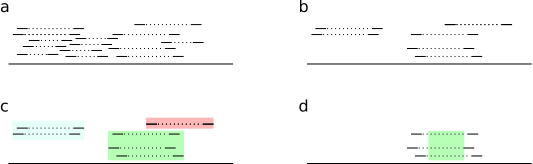
\includegraphics[width=\textwidth]{figures/rp_method_workflow.pdf}
\caption{The general algorithmic steps of a classic read-pair algorithm. a) The algorithm accepts a set of alignments of paired reads to the reference as input. b) The algorithm identifies discordant read pairs. c) Discordant pairs are clustered to find groups that could support the same algorithm. d) Clusters of discordant read pairs are filtered (in this case, by the number of supporting read pairs), and bounds on the potential breakpoints are identified.}
\label{rm_method_workflow}
\end{figure}

A second group of RP methods attempt to include discordant read pairs which cannot be unambiguously mapped to the reference genome in their analysis, in an effort to improve sensitivity in repetitive regions of the genome. One approach to incorporating this type of information can be found in \emph{soft clustering} algorithms, which assign each ambiguously mapped read pair to one of its mappings such that it clusters with other discordant read pairs. These approaches include VariationHunter~\cite{Hormozdiari:2009p284}, which allocates ambiguously mapped reads by optimizing to a maximum parsimony explanation of all discordant reads; HYDRA~\cite{Quinlan:2010gf}, which takes a similar approach based on heuristics, and GASVPro~\cite{Sindi:2012kk}, which uses a Markov-Chain Monte Carlo sampling strategy to assign a read to its correct mapping. Even so, however, most methods use only a limited number of ambiguous discordant mappings per read pair, in part because of the storage and computational requirements necessary to process all or most ambiguous mappings of each read pair in a high-coverage data set.

Finally, CLEVER~\cite{Marschall:2012ek} took an alternative approach and showed that rather than classifying pairs as concordant or discordant and considering only those that are discordant, considering the distribution of all insert sizes allows the detection of smaller events. 

Read pair approaches have the advantage of being theoretically able to detect any type of SV except for multiple copy number duplications. Their disadvantages stem from the fact that they depend on comparing mapping distances between reads to the unknown size of the fragments from which they came. This means that they cannot capture the breakpoints of SVs with single nucleotide resolution, and that they depend on having a sequencing library with a tight distribution of fragment sizes in order to have power.

\section{Read Depth Approaches}

Read-depth (RD) approaches consider the changing depth of coverage of concordantly mapped reads along the genome to infer the presence of SVs. For example, a homozygously deleted region will have zero coverage in the reference genome, while a region that has been duplicated many times, as can happen in some regions of the genome and in some cancers, will have a much higher coverage than average. These approaches differ mainly in the statistical and signal processing techniques used to identify anomalous regions. For example, CNVnator~\cite{Abyzov:2011bk} uses a mean-shift approach to segment the genome into CNV regions. Other approaches in this category include MrFAST~\cite{Alkan:2009cr}, Event-Wise Testing~\cite{Yoon:2009kb}, and SegSeq~\cite{Chiang:2009di}.

RD approaches are good at finding large deletions and duplications. As previously noted, they are the only approach that can identify segments of the genome that have been duplicated multiple times. Their disadvantages are their lack of ability to reliably detect smaller events, and their breakpoint resolution, which is even lower than than of RP approaches.

\section{Split Read Approaches}

Split-read (SR) methods look for breakpoints within individual reads by mapping portions of the read to different genomic locations. Due to the computational challenge involved in aligning reads to the reference genome while allowing for very large gaps between portions of the read, they use different strategies to guide the search. Pindel~\cite{Ye:2009p2} looks for paired reads in which one read in the pair aligned to the reference genome but the other did not. Supposing that the other read may contain a breakpoint, it searches the reference nearby for split read mappings. CREST~\cite{Wang:2011p1607} takes advantage of aligners that insert gaps at the ends of read alignments when there are many mismatches between the read and the reference, known as \emph{soft clipping}. By looking for multiple alignments with soft clips at the same reference coordinate, it can identify breakpoints. 

Split read approaches can identify SVs with high specificity and single base breakpoint accuracy. They are particularly good at detecting smaller variants. However, their sensitivity is limited by coverage and the length of the reads. As read lengths increase with advances in sequencing technology, they will play a larger role in SV detection.

\section{Assembly-Based Approaches}

An alternative approach to mapping reads to the species reference to discover variants is to first attempt to directly assemble the genomic sequence from which the reads were generated (AS approaches). This typically involves the construction of a \emph{de Bruijn} graph to represent the overlapping k-mers in the entire read set, and then walking the graph to construct the longest possible unambiguous sequence of k-mers. Although most work in assembly is focused on \emph{de novo} assembly, when there is no reference for the organism being sequenced, one approach that is targeted at detecting SV's, among other goals, is Cortex~\cite{Iqbal:2012p1837}. Cortex uses the reference to guide assembly with a colored de Bruijn graph structure, and can therefore identify SVs by walking colored paths in its graph.

While AS approaches can theoretically identify any type of SV, in practice assembly requires extremely high coverage (typically 100X). In addition, the computational requirements necessitate high-memory servers, making the task difficult to run on widely available, non-specialized hardware. Finally, genome assembly using short reads tends to collapse identical repeats, leading to a loss of visibililty in repetitive regions of the genome and in segmental duplications\cite{Alkan:2011hs}. Because SVs are enriched in these repetitive regions, this could potentially lead to many false negative calls, and potentially even false positives if repetitive regions are assembled incorrectly, as a loss of a set of repeats could look like a deletion.

\section{Hybrid Approaches}

Recently, approaches have started to appear that try to combine multiple signals in order to improve accuracy. These fall into two groups: those that independently execute more than one of the basic approaches described above and then integrate the results, and those that explicitly create new algorithms to process multiple signals simultaneously.

\subsection{Pipelines}

Pipelines such as SVMerge~\cite{Wong:2010p1271} and HugeSeq~\cite{Lam:2012jy} independently execute multiple algorithms of different types and then attempt to merge the results together. PeSV-Fisher~\cite{Escaramis:2013dm} implements classical RP and RD approaches and then integrates and filters the results. While the integration of these approaches could detect any type of variant detectable by any individual algorithm, it is difficult to combine results from different approaches in a principled manner, and the large number of dependencies and complex parameterization and configuration required has prevented adoption of these pipelines outside of the laboratories in which they were created.

\subsection{Modified Basic Algorithms}

Other tools use one of the four principle approaches outlined above, but have incorporated other signals into their algorithms to improve accuracy. GASVPro~\cite{Sindi:2012kk} is primarily an RP based method, but it used RD signals to validate its predicted breakpoints, assuming that coverage directly around the breakpoint, and in predicted deleted regions, should be reduced. DELLY~\cite{Rausch:2012he} and PRISM~\cite{Jiang:2012cp}, meanwhile, use RP based approaches to identify candidate SV regions, and then guide an SR search for the exact breakpoints of those SVs. Typically, these modifications seem to improve specificity at the expense of sensitivity.

\subsection{Mixtures of Distributions}\label{section_mixture_of_distributions}

Another class of hybrid solution explicitly models the expected number of concordant and discordant pairs at normal and variant locations, effectively combining RP and RD strategies. MoDIL~\cite{Lee:2009da} and the BreakDancerMini component of BreakDancer~\cite{Chen:2009p3} model the distribution of insert sizes at candidate locations in the genome using a Gaussian mixture model. This has two advantages: because reads are not categorized as concordant or discordant based on a hard threshold, it is possible to detect smaller insertions and deletions; and these approaches can explicitly model the zygosity (presence of the variant on one or both of the pairs of chromosomes in the cell) of the variant in the sample, and potentially classify the variant as homozygous or heterozygous. The disadvantage of this approach in these implementations has been the computational requirements, although as we shall see, this strategy lends itself to parallelization. SVMiner~\cite{Hayes:2012ia} follows a somewhat similar approach but does not explicitly model the distribution of insert sizes of read pairs; rather, it created feature vectors based on the number of concordant and discordant read pairs at each locus for deletions, or the number of pairs in each orientation for inversions, and fits a mixture model to the observed distribution of feature vectors across all candidate SVs.

\section{Development of an SV Detection Pipeline for a Cancer Dataset}\label{section_aml_pipeline}

\subsection{Preparation of the Library}

Peripheral blood was collected from a patient with acute myelomonocytic leukemia (previously designated acute myeloid leukemia FAB M4) under a written and oral informed consent process reviewed and approved by the Institutional Review Board of Oregon Health \& Science University. Known cytogenetic abnormalities associated with this specimen included trisomy 8 and internal tandem duplications within the FLT3 gene. Mononuclear cells were separated on a Ficoll gradient, followed by red cell lysis. Mononuclear cells were immunostained using antibodies specific for CD3, CD14, CD34, and CD117 (all from BD Biosciences) and cell fractions were sorted using a BD FACSAria flow cytometer. Cell fractions isolated included T-cells (CD3-positive), malignant monocytes (CD14-positive), and malignant blasts (CD34, CD117-positive). We sequenced CD14+ cells on an Illumina Genome Analyzer II, producing 128,819,200 paired-end reads.

\subsection{Validation of AML Deletions by PCR}

Deletions identified in the AML dataset were validated by PCR. SVs to validate were selected based on calls made by BreakDancer, relying on the score and the number of the reads supporting each single event. Appropriate primers were designed with an internet-based interface, Primer3 \cite{Untergasser01082012}, considering the chromosome localization and orientation of the interval involved in the candidate rearrangement. The primers were checked for specificity using the BLAT tool of the UCSC Human Genome Browser \cite{Kent01042002}. All the primer pairs were preliminarily tested on the patient genomic DNA and a normal genomic DNA as control. The PCR conditions were as follows: 2 min at 95\degree C followed by 35 cycles of 30 sec at 95\degree C, 20 sec at 60\degree C, and 2 min at 72\degree C. All the obtained PCR products were sequenced and analyzed by BLAT for sequence specificity. 

\subsection{Results}

The variants identified include deletions in the gene CTDSPL/RBPS3, an AML tumor suppressor~\cite{Zheng:2012kk}, and NBEAL1, a gene up-regulated in some cancers~\cite{Chen:2004jo}. We are currently investigating these deletions to determine their functional impact on this patient. 

\chapter{A General Framework for SV Detection in MapReduce}\label{chap_framework}

MapReduce~\cite{Dean:2008p277} divides computation across a cluster into three phases. In the first phase, \emph{mappers} developed by the application programmer examine small blocks of data and emit a set of $\langle key, value \rangle$ pairs for each block examined. The MapReduce framework then sorts the output of the mappers by key, and aggregates all values that are associated with each key. Finally, the framework executes \emph{reducers}, also created by the application developer, which process all of the values for a particular key and produce one or more outputs that summarize or aggregate those values. MapReduce and Hadoop allow efficient processing of large data sets by scheduling tasks for execution as close as possible to the nodes which hold the required data, minimizing network traffic and I/O contention.

The need to separate logic into mappers and reducers makes it difficult to implement traditional RP-based SV detection approaches in MapReduce, particularly given the global clustering of paired end mappings at the heart of many RP approaches. MapReduce algorithms, by contrast, excel at conducting many independent calculations in parallel. The sequencing applications that have been implemented in MapReduce succeed by dividing processing into a series of local computation, for example calling a SNV at a particular location in the genome given the reads that cover it, which is the approach taken by the variant callers GATK~\cite{McKenna:2010p1051} and Crossbow~\cite{Langmead:2009p1225}. SV approaches that are similarly based on local computations have been described: the RP-based SV callers MoDIL~\cite{Lee:2009da} and forestSV~\cite{Michaelson:2012fj} try to solve the SV detection problem by computing scores or features along the genome and then producing SV predictions from those features in a post-processing step. 

Using this strategy, we have developed a conceptual algorithmic framework for SV detection in MapReduce, which is outlined in Algorithm~\ref{cb_algo}. This framework divides processing into three separate MapReduce jobs: an alignment job, a feature computation job, and an SV calling job. The overall workflow of the algorithm and its implementation on a compute cluster or cloud is summarized in Figure~\ref{cloudbreak_workflow}.

\begin{figure}
\centering
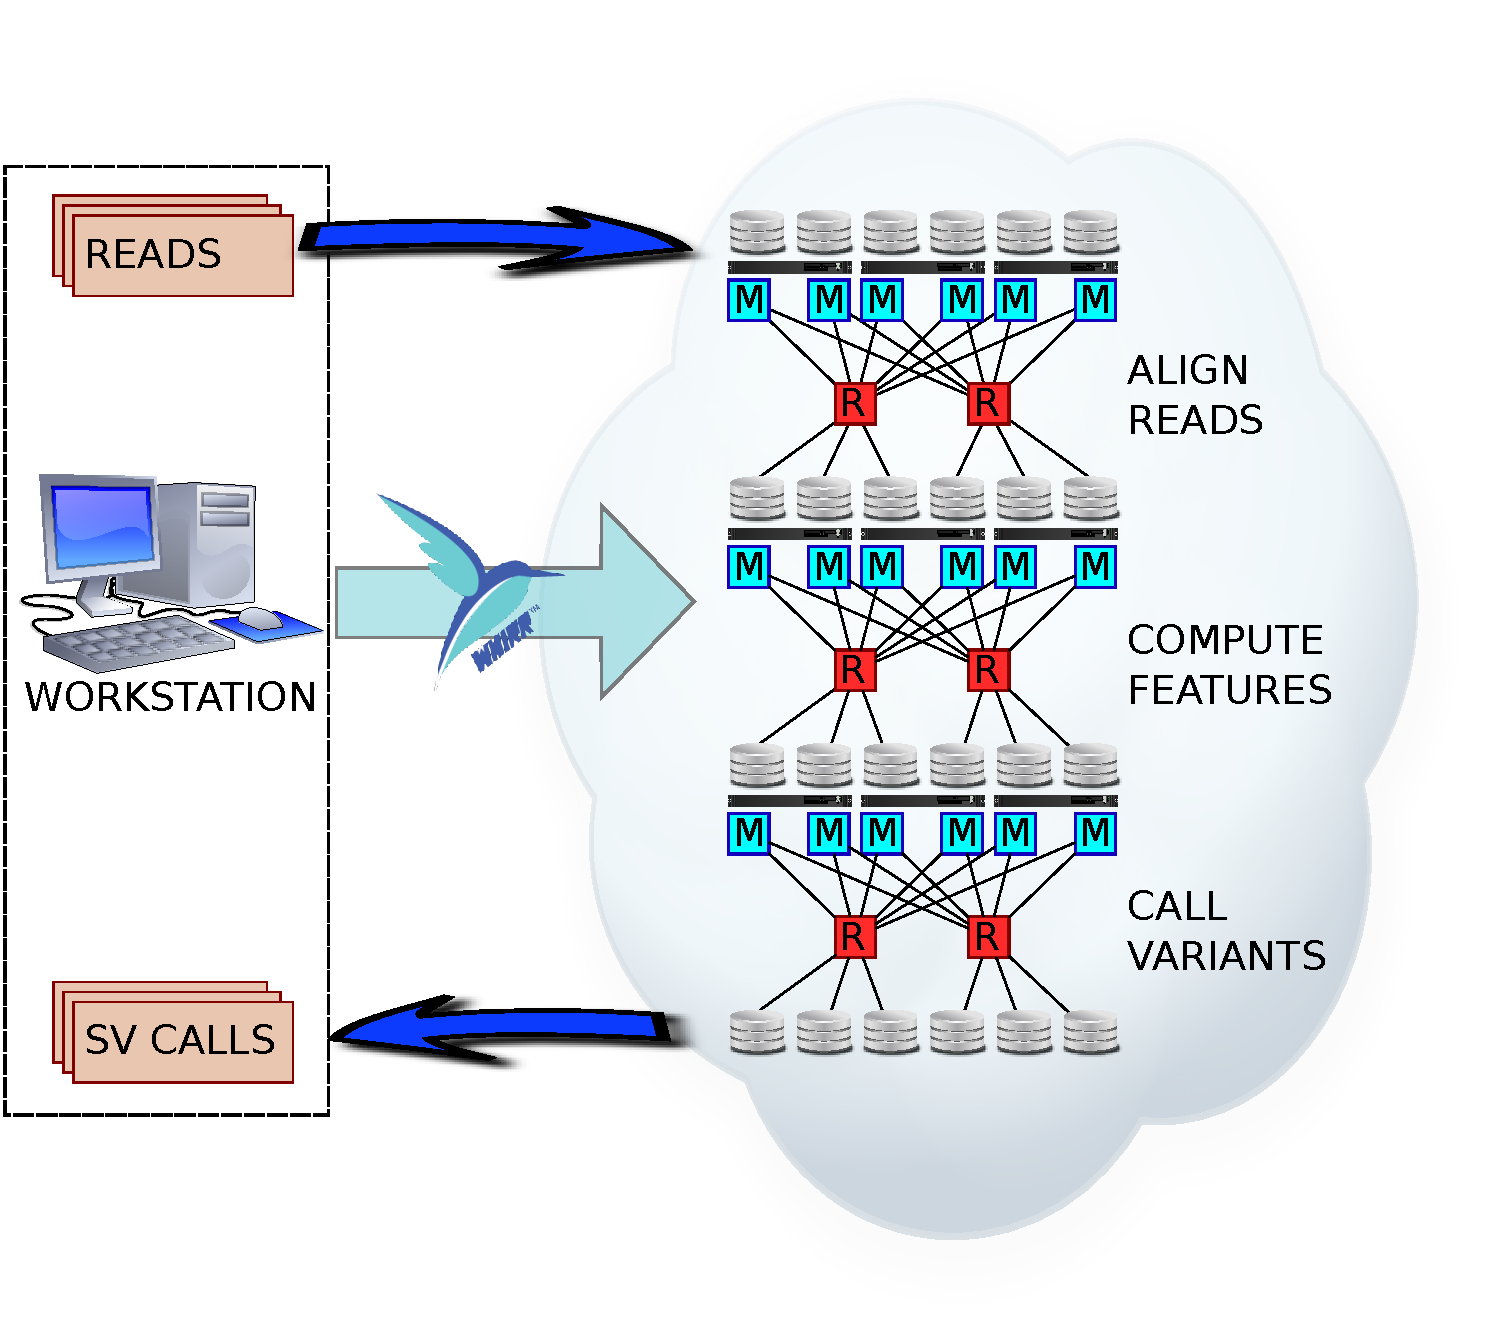
\includegraphics[width=.8\textwidth]{figures/workflow_with_whirr.png}
\caption{An overview of the Cloudbreak workflow. Reads are first uploaded to a Hadoop cluster from local storage. Cloudbreak then executes three MapReduce jobs to process the data: 1) Mapping with sensitive settings. 2) Computation of features across the genome. 3) Calling structural variations based on the features computed in the previous step. Finally, SV predictions can be downloaded from the Hadoop cluster and examined. Cloudbreak can also use the Apache Whirr library to automatically provision Hadoop clusters on and deploy data to cloud providers such as Amazon Elastic Compute Cloud.}
\label{cloudbreak_workflow}
\end{figure}


The \textsc{Align Reads} job uses existing alignment tools to discover mapping locations for each read pair. Aligners can be executed to report multiple possible mappings for each read, or only the best possible mapping. Given a set of read pairs, each of which consists of a read pair identifier $rpid$ and two sets of sequence and quality scores $<s,q>$, each mapper aligns each pair end set $<s,q>$ in either single- or paired end mode and emits possible mapping locations under the $rpid$ key. Reducers then collect the alignments for each paired end, making them available under one key for the next job. Our implementation of the framework contains wrappers to execute the aligners BWA \cite{Li:2009p836}, GEM \cite{MarcoSola:2012hm}, Novoalign \cite{novoalign}, RazerS 3 \cite{Weese:2012by}, mrFAST \cite{Alkan:2009cr}, and Bowtie 2 \cite{Langmead:2012jh}. This job can also be skipped in favor of importing a pre-aligned BAM file directly into HDFS.

In the \textsc{Compute Features} job, we compute a set of features for each location in the genome. To begin, we tile the genome with small fixed-width, non-overlapping intervals. For the experiments reported in this paper we use an interval size of 25bp. Let $L = \left\{l_1,l_2,\ldots,l_N\right\}$ be the set of intervals covering the entire genome. Let $R^1 = \left\{r^{1}_{1},r^{1}_{2},\ldots,r^{1}_{M}\right\}$ and $R^2 = \left\{r^{2}_{1},r^{2}_{2},\ldots,r^{2}_{M}\right\}$ be the input set of paired reads. Let $A^1 = \left\{a^{1}_{m,1},a^{1}_{m,2},\ldots,a^{1}_{m,K}\right\}$ and $A^2 = \left\{a^{2}_{m,1},a^{2}_{m,2},\ldots,a^{2}_{m,L}\right\}$ be the set of alignments for the left and right reads from read pair $m$. For any given pair of alignments of the two reads in a read pair, $a^{1}_{m,i}$ and $a^{2}_{m,j}$, let the $\textrm{ReadPairInfo } rpi_{m,i,j}$ be information about the pair relevant to detecting SVs, e.g. the fragment size implied by the alignments and the likelihood that the alignments are correct. We then leave two functions to be implemented depending on the application:
\begin{flalign*}
 \textsc{Loci } :& \langle a^{1}_{m,i},a^{2}_{m,j} \rangle \rightarrow L_m \subseteq L \\
 \Phi :& \left\{\textrm{ReadPairInfo }rpi_{m,i,j}\right\} \rightarrow \mathbb{R}^N \\
\end{flalign*}

The first function, \textsc{Loci}, maps an alignment pair to a set of genomic locations to which it is relevant for SV detection; for example, the set of locations overlapped by the internal insert implied by the read alignments.  We optimize this step by assuming that if there exist concordant mappings for a read pair, defined as those where the two alignments are in the proper orientation and with an insert size within three standard deviations of the expected library insert size, one of them is likely to be correct and therefore we do not consider any discordant alignments of the pair. The second function, $\Phi$, maps a set of ReadPairInfos relevant to a given location to a set of real-valued vectors of features useful for SV detection. 

Finally, the third MapReduce job, \textsc{Call Variants}, is responsible for making SV calls based on the features computed at each genomic location. It calls another application-specific function  $\textsc{PostProcess} : \left\{\phi_1,\phi_2,\ldots,\phi_N\right\} \rightarrow \left\{\langle  \textrm{SVType } s, l_{start}, l_{end} \rangle\right\}$  that maps the sets of features for related loci into a set of SV calls characterized by their type $s$ (i.e Deletion, Insertion, etc.) and their breakpoint locations $l_{start}$ and $l_{end}$. We parallelize this job in MapReduce by making calls for each chromosome in parallel, which we achieve by associating a location and its set of features to its chromosome in the map phase, and then making SV calls for one chromosome in each reduce task.

\begin{algorithm}[h]
\algrenewcommand\algorithmicprocedure{\textbf{job}}
 \begin{algorithmic}[1]
 \Procedure{Alignment}{}
 \Function{Map}{$\textrm{ReadPairId }rpid, \textrm{ReadId }r, \textrm{ReadSequence }s, \textrm{ReadQuality }q$}
 \ForAll{$ \textrm{Alignments }a \in \textsc{Align}(<s,q>)$}
 \State $\textsc{Emit}(\textrm{ReadPairId }rpid, \textrm{Alignment }a)$
 \EndFor
 \EndFunction
 \Function{Reduce}{$\textrm{ReadPairId }rpid, \textrm{Alignments }a_{1,2,\ldots}$}
 \State $\textrm{AlignmentPairList }ap \gets \textsc{ValidAlignmentPairs}(a_{1,2,\ldots})$
 \State $\textsc{Emit}(\textrm{ReadPairId }rp, \textrm{AlignmentPairList } ap)$
 \EndFunction
 \EndProcedure

 \Procedure{Compute SV Features}{}
 \Function{Map}{$\textrm{ReadPairId }rp, \textrm{AlignmentPairList }ap$}
 \ForAll{$ \textrm{AlignmentPairs }<a_1,a_2> \in ap$}
 \ForAll{$ \textrm{GenomicLocations }l \in \textsc{Loci }(a_1,a_2)$}
 \State $ \textrm{ReadPairInfo }rpi \gets <\textrm{InsertSize}(a_1,a_2), \textrm{AlignmentScore}(a_1,a_2)>$
 \State $\textsc{Emit}(\textrm{GenomicLocation }l, \textrm{ReadPairInfo }rpi)$
 \EndFor
 \EndFor
 \EndFunction
 \Function{Reduce}{$\textrm{GenomicLocation }l, \textrm{ReadPairInfos }rpi_{1,2,\ldots}$}
 \State $\textrm{SVFeatures } \phi_l \gets \Phi(\textrm{InsertSizes }i_{1,2,\ldots}, \textrm{AlignmentScores }q_{1,2,\ldots})$
 \State $\textsc{Emit}(\textrm{GenomicLocation }l, \textrm{SVFeatures } \phi_l)$
 \EndFunction
 \EndProcedure

 \Procedure{Call SVs}{}
 \Function{Map}{$\textrm{GenomicLocation }l, \textrm{SVFeatures } \phi_l$}
 \State $\textsc{Emit}(\textrm{Chromosome}(l), <l,\phi_l>)$
 \EndFunction
 \Function{Reduce}{$\textrm{Chromosome }c, \textrm{GenomicLocation } l_{1,2,\ldots},\phi_{1,2,\ldots}$}
 \State $\textrm{StructuralVariationCalls } svs_c \gets \textsc{PostProcess }(\phi_{1,2,\ldots})$
 \EndFunction
 \EndProcedure
 \end{algorithmic}
\caption{The algorithmic framework for SV calling in MapReduce.}
\label{cb_algo}
\end{algorithm}


\chapter{Cloudbreak}\label{chap_cloudbreak_impl}

In the previous chapter, we described and formalized a general strategy for building SV detection algorithms in MapReduce and Hadoop. In this chapter, we describe an software package, Cloudbreak, that we have developed using this algorithmic framework. To build Cloudbreak, we implemented the infrastructure necessary to support the algorithmic framework we described in Section~\ref{section_general_algo}, and also provided implementations of the three application-specific functions we described there. Here we will describe this implementation, as well as our choices for the three user-defined functions we specified in the framework definition, and additional functionality we developed to genotype calls and to facilitate the deployment of Cloudbreak on public cloud platforms including Amazon's EC2. In Chapter~\ref{chap_cloudbreak_eval}, we will provide an evaluation of the algorithm's accuracy and performance characteristics.

\section{Variant types detected}

Cloudbreak is our implementation of a detection algorithm for genomic deletions (40bp-25,000bp) and small insertions based on examining the insert sizes of paired end mappings. We chose this application because small deletions in the range of 50bp to 150bp are particularly difficult to detect using many existing SV algorithms~\cite{Alkan:2011p547,Mills:2011fi}. This is because most read-pair based algorithms use a hard cutoff based on the variance of the fragment size distribution to select discordant read pairs, as described in Section~\ref{section_read_pair}. By taking advantage of many compute cores using MapReduce, we can design an algorithm that considers all of available data (both concordant and discordant read pairs) in a generative statistical framework, as we will describe in Section~\ref{section_user_defined_functions}.

\section{Framework infrastructure}

In addition to the specific algorithm for detecting deletions and insertions (which take the form of implementations of the user-defined functions we described in the previous chapter), the Cloudbreak package also contains the infrastructure necessary to implement the three MapReduce jobs defined in our MapReduce algorithmic framework. Providing a fully featured, multi-job Hadoop application requires several implementation decisions:

\begin{itemize}
\item \textbf{Programming language and method of interacting with Hadoop.} Hadoop applications can be developed in several ways. A native application is written in Java and directly uses the Hadoop application programming interface (API) to start jobs, implement Map and Reduce functions, and set advanced Hadoop configurations. Alternatively, applications can be developed in any language using the Hadoop \emph{streaming} interface, as long as the input to and output from all map and reduce tasks is textual and certain conventions are followed with respect to data format. Finally, for C/C++ applications, the Hadoop \emph{pipes} interface can be used to marshal input and output data from tasks. Each method has its own advantages and disadvantages. Native applications constrain the developer to Java but enjoy the best performance when the jobs are data intensive rather than CPU bound~\cite{Ding:2011:MCM:2103380.2103444}. Streaming applications allow greater programming language flexibility but make it somewhat more difficult to organize complex applications and take advantage of advanced Hadoop features. Pipes, meanwhile, allow for maximum performance for CPU intensive applications. We opted to develop Cloudbreak as a native application to take advantage of the tight integration with the Hadoop API improved I/O performance on data intensive portions of the workflow. For the \textsc{Align Reads} job, which executes existing short-read alignment tools, a mapper class written in Java invokes the external tools using the system runtime environment.

\item \textbf{File formats and compression.} Hadoop applications usually store their data in HDFS in text format or in sequence files, a binary format that allows numeric or complex data types to be stored in a key-value pair structure easily accessed by Hadoop. In addition, varying levels of compression can be used, although only certain compression types allow Hadoop to automatically split large files by HDFS blocks for processing by different map tasks, which is a key consideration for building fully parallelized applications. Cloudbreak uses sequence files for input and intermediate files, although for alignments the values are stored as text strings containing full records in the Sequence Alignment Map (SAM) format~\cite{Li:2009vz}, to allow for easy exports of data. For compression we use the Snappy~\cite{snappy} compressor/decompressor (codec), a compression scheme developed at Google which aims for reasonable file size reduction with very fast compression and decompression speeds. This makes it ideal for data-intensive Hadoop applications. Given that the output data from the \textsc{Align Reads} job is alignment records, a future implementation goal is to switch to using Hadoop-BAM~\cite{Niemenmaa:2012hu}, a library for storing SAM/BAM records efficiently in HDFS; Hadoop-BAM did not posses necessary functionality at the time of Cloudbreak's initial implementation and so we proceeded with a text-based representation of alignment records.

\item \textbf{Distribution of auxiliary files.} In some cases all tasks require access to large input files, such as genome reference indices for alignment, or genome annotation files. Hadoop offers a \emph{distributed cache} service, which places copies of the files on each node that will host tasks for the job so that they will not all need to copy the files over the network. Cloudbreak makes use of the distributed cache to distribute index and annotation files, as well as the alignment executables for the \textsc{Align Reads} job.
\end{itemize}

Our implementation of the \textsc{Align Reads} job contains wrappers to execute the aligners BWA \cite{Li:2009p836}, GEM \cite{MarcoSola:2012hm}, Novoalign \cite{novoalign}, RazerS 3 \cite{Weese:2012by}, mrFAST \cite{Alkan:2009cr}, and Bowtie 2 \cite{Langmead:2012jh}. This job can also be skipped in favor of importing a pre-aligned BAM file directly into HDFS. The code is structured in such a way that to add a new aligner, developers would simply create a class that finds the necessary index files in the distributed cache and determines the proper command line parameters for aligner execution, and parses the aligner output if it is in a non-standard format.

Cloudbreak can be executed on any Hadoop cluster; Hadoop abstracts away the details of cluster configuration, making distributed applications portable. We deployed Cloudbreak on an internal 56-node cluster running the Cloudera CDH3 Hadoop distribution, version 0.20.2-cdh3u4. In addition, Cloudbreak can create and operate on Hadoop clusters in the Amazon compute cloud (see Section~\ref{section_cloud_whirr}).

\section{Implementation of a MapReduce SV Algorithm}\label{section_user_defined_functions}

In Section~\ref{section_general_algo}, we described three user-defined functions that can be implemented to create an SV detection application in our MapReduce framework. These functions were named \textsc{Loci}, $\Phi$, and \textsc{PostProcess}. These functions map aligned read pairs to locations on the genome to which they are relevant, compute a set of local features for each genomic location based on the relevant read pairs, and call variants based on the features computed for neighboring genomic locations. Cloudbreak contains implementations of these functions that combine to allow it to detect deletions (of size 40bp-25,000bp) and insertions. A detailed description of each of these implementations appears below, and an illustration of each phase of the Cloudbreak algorithm working on a simple example in MapReduce is shown in Figure \ref{cloudbreak_example}.

\begin{figure}
\centering
\includegraphics[width=.9\textwidth]{/users/cwhelan/Documents/svpipeline/figures/cloudbreak_mapred_diagram.pdf}
\caption{An Example of the Cloudbreak deletion and insertion detection algorithm running in MapReduce. A) In the first MapReduce job, mappers scan input reads in FASTQ format and execute an alignment program in either paired-end or single-ended mode to generate read mappings. Reducers gather all alignments for both reads in each pair. B) In the second MapReduce job, mappers first emit information about each read pair (in this case the insert size and quality) under keys indicating the genomic location spanned by that pair. Only one genomic location is diagrammed here for simplicity. Reducers then compute features for each location on the genome by fitting a GMM to the distribution of spanning insert sizes. C) Mappers group all emitted features by their chromosome, and reducers find contiguous blocks of features that indicate the presence of a variant.}
\label{cloudbreak_example}
\end{figure}

\begin{description}
\item[\sc{Loci}] Because we are detecting deletions and short insertions, we map ReadPairInfos from each possible alignment to the genomic locations overlapped by the implied internal insert between the reads. For efficiency, we define a maximum detectable deletion size of 25,000bp, and therefore alignment pairs in which the ends are more than 25kb apart, or in the incorrect orientation, map to no genomic locations. In addition, if there are multiple possible mappings for each read in the input set, we optimize this step by assuming that if there exists a concordant mapping for a read pair, defined as a mapping pair in which the two alignments are in the proper orientation and with an insert size within three standard deviations of the expected library insert size, it is likely to be correct and therefore we do not consider any discordant alignments of the pair.

\item[$\Phi$] To compute features for each genomic location, we follow the mixture of distributions approach (see Section~\ref{section_mixture_of_distributions}) first described by Lee et al.~\cite{Lee:2009da}, who observed that if all mappings are correct, the insert sizes implied by mappings which span a given genomic location should follow a Gaussian mixture model (GMM) whose parameters depend on whether a deletion or insertion is present at that locus. Figure~\ref{insert_size_mixes} shows several examples of the mixtures observed for various types of variants. If there is no indel, the insert sizes implied by spanning alignment pairs should follow the distribution of actual fragment sizes in the sample, which is typically modeled as normally distributed with mean $\mu$ and standard deviation $\sigma$. If there is a homozygous deletion or insertion of length $l$ at the location, $\mu$ should be shifted to $\mu + l$, while $\sigma$ will remain constant. Finally, in the case of a heterozygous event, the distribution of insert sizes will follow a mixture of two normal distributions, one with mean $\mu$, and the other with mean $\mu + l$, both with an unchanged standard deviation of $\sigma$, and mixing parameter $\alpha$ that describes the relative weights of the two components. The features generated for each location $l$ include the log-likelihood ratio of the filtered observed data points under the fit GMM to their likelihood under the distribution $N(\mu,\sigma)$, the final value of the mixing parameter $\alpha$, and $\mu'$, the estimated mean of the second GMM component. 

The choice of a mixture of distributions model has several benefits. Firstly, it is a generative model for the entire data set, including concordant and discordant read pairs. This removes the need to set hard thresholds that define discordant read pairs, and allows the detection of smaller variants given a tight enough insert size distribution. Second, the parameters that are estimated can be used to refine and classify predictions. For example, the mixing parameter $\alpha$ can be used to genotype variants, as we will describe in Section~\ref{section_genotyping}. In addition, the estimated $\mu'$ parameter gives a prediction for how many genomic locations the variant might cover, which we leverage in the \textsc{PostProcess} function described below to integrate local features into variant calls.

To implement our model, at each genomic location we fit the parameters of the GMM using the Expectation-Maximization algorithm. Let $Y = y_{1,2, \ldots m}$ be the observed insert sizes at each location after filtering, and say the library has mean fragment size $\mu$ with standard deviation $\sigma$. Because the mean and standard deviation of the fragment sizes are selected by the experimenter and therefore known \emph{a priori} (or at least easily estimated based on a sample of alignments), we only need to estimate the mean of the second component at each locus, and the mixing parameter $\alpha$. Therefore, we initialize the two components to have means $\mu$ and $\bar{Y}$, set the standard deviation of both components to $\sigma$, and set $\alpha = .5$. In the E step, we compute for each $y_i$ and GMM component $j$ the value $\gamma_{i,j}$, which is the normalized likelihood that $y_i$ was drawn from component $j$. We also compute $n_j = \sum_i{\gamma_{i,j}}$, the relative contributions of the data points to each of the two distributions. In the M step, we update $\alpha$ to be $n_2 - \left|Y\right|$, and set the mean of the second component to be $\frac{\sum_m{\gamma_{m,2}y_m}}{n_2}$. We treat the variance as fixed and do not update it, since under our assumptions the standard deviation of each component should always be $\sigma$. We repeat the E and M steps until convergence, or until a maximum number of steps has been taken. Prior to fitting the GMM at each location, we attempt to filter out incorrect mappings for that location using an outlier-detection based clustering scheme and an adaptive mapping quality cutoff; see Section~\ref{section_incorrect_and_ambiguous_mappings} for details.

\item[\sc{PostProcess}] The third MapReduce job is responsible for making SV calls based on the features defined above. We convert our features along each chromosome to insertion and deletion calls by first extracting contiguous genomic loci where the log-likelihood ratio of the two models is greater than a given threshold. To eliminate noise we apply a median filter with window size 5. We end regions when $\mu'$ changes by more than 60bp ($2\sigma$), and discard regions where the average value of $\mu'$ is less than $\mu$ or where the length of the region differs from $\mu'$ by more than $\mu$.
\end{description}

\begin{figure}
\centering
\includegraphics[width=.9\textwidth]{figures/insert_size_mixtures.pdf}
\caption{Illustration of insert size mixtures at individual genomic locations. A) there is no variant present at the location indicated by the vertical line (left), so the mix of insert sizes (right) follows the expected distribution of the library centered at 200bp, with a small amount of noise coming from low-quality mappings. B) a homozygous deletion of 50bp at the location has shifted the distribution of observed insert sizes. C) A heterozygous deletion at the location causes a mixture of normal and long insert sizes to be detected. D) A heterozygous small insertion shifts a portion of the mixture to have lower insert sizes.}
\label{insert_size_mixes}
\end{figure}

\section{Filtering Incorrect and Ambiguous Mappings}\label{section_incorrect_and_ambiguous_mappings}

To handle incorrect and ambiguous mappings, we assume that in general they will not form normally distributed clusters in the same way that correct mappings will, and therefore use an outlier detection technique to filter the observed insert sizes for each location. We sort the observed insert sizes and define as an outlier an observation whose $k$th nearest neighbor is more than $n\sigma$ distant, where $k = 3$ and $n = 5$. In addition, we rank all observations by the estimated probability that the mapping is correct and use an \emph{adaptive quality cutoff} to filter observations: we discard all observations where the estimated probability the mapping is correct is less than the score of the maximum quality observation minus a constant $c$. This allows the use of more uncertain mappings in repetitive regions of the genome while restricting the use of low-quality mappings in unique regions. Defining $\textsc{Mismatches}(a)$ to be the number of mismatches between a read and the reference genome in the alignment $a$, we approximate the probability $p^{k}_c$ of each end alignment being correct by:

\[ p^{k}_c(a^{k}_{m,i}) = \frac{\exp({-\textsc{Mismatches}(a^{k}_{m,i})/2)}}{\sum_j{\exp(-\textsc{Mismatches}(a^{k}_{m,j})/2)}} \]

And then multiply $p_c(a^{1}_{m,i})$ and $p_c(a^{2}_{m,i})$ to approximate the likelihood that the pair is mapped correctly.

\section{Genotyping}\label{section_genotyping}

In theory, it should be possible to use the parameters of the fit GMM to infer the genotype of each predicted variant. Assuming that our pipeline is capturing all relevant read mappings near the locus of the variant, the genotype should be indicated by the estimated parameter $\alpha$, the mixing parameter that controls the weight of the two components in the GMM.  We set a simple cutoff on the average value of $\alpha$ for each prediction to call the predicted variant homozygous or heterozygous, and use the same cutoff for deletion and insertion predictions. Somewhat surprisingly, we observed on the cutoff point that distinguishes homozygous from heterozygous variants is significantly less than the expected .5; based on empirical observations on a simulated data set, we set the threshold to .35 (see Section~\ref{section_genotyping_eval} for more details).

\section{Running in the Cloud}\label{section_cloud_whirr}

The need for tools that ease the use of cloud resources has recently been recognized by the genomics community~\cite{Schatz:2010js,Stein:2010gp}, spurring the development of a variety of applications and toolkits that use the APIs of Infrastructure as a Service (IaaS) providers, such as Amazon EC2, to allocate compute resources on public compute clouds. We will review some of the existing cloud-enabled tools, including those that are based on traditional grid scheduling engines and those that enable Hadoop and MapReduce pipelines. Many of the latter take advantage of Amazon's Elastic MapReduce (EMR) service, an offering from Amazon specifically for creating and running Hadoop jobs that simplifies the creation and monitoring of clusters on EC2. We will then discuss how Cloudbreak enables the use of cloud computing in a provider-neutral way using the Apache Whirr library.

\subsection{Other Cloud-Enabled Genomics Tools}

For example, the CloudBioLinux project~\cite{Krampis:2012wo} provides virtual machine images for use in Amazon EC2 that are pre-configured with a wide range of open-source bioinformatics applications. Galaxy CloudMan~\cite{Afgan:2010fa} allows for the automatic creation of clusters in the Amazon cloud configured to run workflows in the popular Galaxy environment~\cite{Giardine:2005ig}, backed by the SGE grid scheduling engine and with interfaces to Amazon's S3 storage service. CloVR~\cite{Angiuoli:2011wl} is a newer cloud cluster manager that includes several pipelines for metagenomics managed by SGE. Finally, Elastream~\cite{Issa:2013jp} is a newer offering that can provision and manage cloud clusters using either grid schedulers or EMR. 

Several commercial providers are also offering services that allow elastic cloud computing for sequencing pipelines, including DNAnexus (Mountain View, CA), Illumina's (San Diego, CA) BaseSpace cloud, Seven Bridges Genomics' (Cambridge, MA) IGOR platform, and an offering from Biodatomics (Bethesda, MD). These commercial cloud services are in many cases backed by Amazon's EC2, but are wrapped in additional sequencing-specific APIs and user interfaces by the vendor. To our knowledge Biodatomics is the only commercial bioinformatics vendor that offers automatic Hadoop cluster provisioning, however. 

There are also a number of bioinformatics suites designed for specific applications that are able to allocate resources on EC2 automatically. Apart from those that use Hadoop, which we will discuss shortly, these include: Atlas2 Cloud~\cite{Evani:2012eq}, which allows users to run the Genboree Workbench workflow for variant calling and annotation in personal genomics DNA resequencing projects; SIMPLEX~\cite{Fischer:2012bt}, which enables cloud processing for an exome alignment and variant calling pipeline based on BWA and the GATK; a set of ChIP-seq tools of the modENCODE and ENCODE projects~\cite{Trinh:2013ii} that can create clusters to run analysis pipelines on EC2 or the Bionumbus private cloud~\cite{bionimbus}.

Finally, several of the Hadoop applications we discussed in Section~\ref{section_mapred_related_work} come with command-line or graphical interfaces that automate their deployment on commercial cloud services. Most of these leverage EMR. The most widely used EMR-enabled tool is Crossbow~\cite{Langmead:2009p1225}, which has a UI that will create Hadoop workflows using EMR. Crossbow's ability to use EMR was recently made more robust by Rainbow~\cite{Zhao:2013hj}, which wraps Crossbow with additional facilities for transferring large files in parallel, monitoring clusters for failing nodes, and aggregating results from multiple samples run simultaneously. As mentioned in Section~\ref{section_mapred_related_work}, FX~\cite{Hong:2012du} and Euolsan~\cite{Jourdren:2012dc} are both Hadoop workflows for RNA-seq processing; both have the ability to automatically create EMR jobs on Amazon EC2.

\subsection{Enabling Cloud Computing with Whirr}

Cloudbreak leverages the Apache Whirr~\cite{whirr} library to automatically create clusters with cloud service providers. Whirr differs from the strategies referred to in the last section in that Whirr provides a unified application programming interface (API) for provisioning and running cloud services that is agnostic to the cloud IaaS provider. Although the largest and most popular cloud IaaS is provided by Amazon Web Services though their Elastic Compute Cloud (EC2), Whirr provides a facade API that allows the transparent substitution of other cloud services such as Rackspace, Microsoft Azure, or private clouds such as those built with Eucalyptus. Most of the Hadoop-enabled applications and toolkits mentioned in the previous section depend on Amazon Elastic MapReduce to provision Hadoop clusters. Cloudbreak's use of Whirr breaks this dependency on a single vendor.

Using Whirr's API, Cloudbreak can provision of Hadoop clusters which can then be terminated when processing is complete. This eliminates the need to invest in a standing cluster and allows a model in which users can scale their computational infrastructure as their need for it varies over time. Through a command line interface, Cloudbreak uses Whirr functionality to offer commands that:

\begin{itemize}
\item \textbf{Automatically provision Hadoop clusters in the cloud.} After specifying the parameters of the Hadoop cluster desired in a property file, a single Cloudbreak command will request the creation of the necessary compute instances in the cloud, will configure them with the proper Hadoop services to provide a fully functioning cluster, and will start proxies that make the Hadoop cluster's management and reporting UIs available to the user. Cloudbreak users can configure clusters with their credentials for the cloud service provider, the number of worker nodes to include in the cluster as well the hardware requirements for each node, and, if desired, the pricing model. This last point is particularly useful on EC2, where spot pricing allows users to bid for unclaimed compute capacity on Amazon's cloud. Spot pricing can dramatically reduce costs compared to full price on-demand instances. The disadvantage is that instances can be reallocated if a higher bid comes in, resulting in termination of the processes they are running. Hadoop's facility for automatic redundancy of data and tasks can mitigate this risk.

\item \textbf{Transfer data into cloud compute clusters.} Typically when using cloud compute services it is fastest to store large data sets in a cloud storage service such as Amazon's Simple Storage Service (S3). From there it is fast to transfer them into and out of cloud compute services like EC2. However, moving data into S3 can be time-consuming depending on the network connections and number and size of the files in the data set. Cloudbreak includes code which communicates with S3 to do a multi-threaded upload of large data files, enabling much faster transfer times.

\item \textbf{Destroy clusters when processing is complete.} Cloudbreak, by using the Whirr API, can destroy allocated cloud clusters when processing is complete, ensuring that compute costs can be managed efficiently.
\end{itemize}

Cloudbreak's user manual contains detailed instructions and examples describing how to leverage cloud computing. We hope that by making cloud computing readily accessible through Cloudbreak's command line interface, more researchers will have the opportunity to leverage Hadoop's distributed computing model, even if they do not have local Hadoop clusters available at their institutions.

\section{Discussion}

The GMM-based mixture of distributions approach has been used by the SV detection tools MoDIL~\cite{Lee:2009da}, SVMiner~\cite{Hayes:2012ia}, and SVM$^2$~\cite{Chiara:2012ey}. However, SVMiner only models mixtures of distributions for candidate regions that have been identified through a traditional discordant pair analysis. This removes the benefit of being able to use the GMM to identify smaller variants. Similarly, SVM$^2$ fits a mixture of distributions only to candidate regions of the genome identified through a preliminary analysis. This leaves MoDIL as the only tool that attempts to model the distribution of insert sizes across the entire genome. As we will see in the next chapter, MoDIL is prone to excessively long run times that make it impractical to run for large-scale genomics data sets. Cloudbreak, on the other hand, is able to efficiently leverage compute clusters to be able to deliver the benefits of this strategy with very fast runtimes.

For those researchers that wish to take advantage of cloud computing in order to avoid the expense and maintenance costs of running their own large Hadoop clusters, Cloudbreak is able to automatically provision, transfer data to, and destroy Hadoop clusters using IaaS providers. Although there are other cloud-enabled sequencing analysis tools, Cloudbreak is unique in using the Apache Whirr library to provide an IaaS provider-agnostic solution. In addition to the obvious benefit of avoiding vendor lock-in, we believe that this will become increasingly important in the future as research agencies and clinical providers increasingly set up private or semi-private clouds to manage the analysis of sensitive personal genomic data in a controlled setting.

\chapter{Evaluation}\label{chap_cloudbreak_eval}

\section{Choice of Methods to Compare To}

We compared the performance of Cloudbreak for detecting deletions and insertions to a selection of popular tools: the RP method BreakDancer \cite{Chen:2009p3}, GASVPro, an RP method that integrates RD signals and ambiguous mappings \cite{Sindi:2012kk}, the SR method Pindel \cite{Ye:2009p2}, and the hybrid RP-SR method DELLY \cite{Rausch:2012he}. DELLY produces two sets of calls, one based solely on RP signals, and the other based on RP calls that could be supported by SR evidence; we refer to these sets of calls as DELLY-RP and DELLY-SR. We also attempted to evaluate MoDIL on the same data. All of these methods detect deletions. Insertions can be detected by BreakDancer, Pindel, and MoDIL. 

Simulated reads were aligned to hg18 chromosome 2, and NA18507 reads were aligned to the hg19 assembly. Alignments for all programs, unless otherwise noted, were aligned using BWA \texttt{aln} version 0.6.2-r126, with parameter \texttt{-e 5} to allow for longer gaps in alignments due to the number of small indels near the ends of larger indels in the Venter data set. GASVPro also accepts ambiguous mappings; we extracted read pairs that did not align concordantly with BWA and re-aligned them with Novoalign V2.08.01, with parameters \texttt{-a -r -Ex 1100 -t 250}. 

We ran BreakDancer version 1.1\_2011\_02\_21 in single threaded mode by first executing \texttt{bam2cfg.pl} and then running \texttt{breakdancer\_max} with the default parameter values.  To run Breakdancer in parallel mode we first ran \texttt{bam2cfg.pl} and then launched parallel instances of \texttt{breakdancer\_max} for each chromosome using the \texttt{-o} parameter. We ran DELLY version 0.0.9 with the \texttt{-p} parameter and default values for other parameters. For the parallel run of DELLY we first split the original BAM file with BamTools \cite{Barnett:2011hm}, and then ran instances of DELLY in parallel for each BAM file. We ran GASVPro version 1.2 using the \texttt{GASVPro.sh} script and default parameters. Pindel 0.2.4t was executed with default parameters in single CPU mode, and executed in parallel mode for each chromosome using the \texttt{-c} option. We executed MoDIL with default parameters except for a \texttt{MAX\_DEL\_SIZE} of 25000, and processed it in parallel on our cluster with a step size of 121475. To execute parallelize other SV detection tools we wrote simple scripts to submit jobs to the cluster using the HTCondor scheduling engine \cite{condor} with directed acyclic graphs to describe dependencies between jobs. 


\section{A Note on Comparing and Evaluating Performance and Runtime}

We implemented and executed Cloudbreak on a 56-node Hadoop cluster, with 636 map slots and 477 reduce slots. Not including alignment time, we were able to process the Chromosome 2 simulated data in under five minutes, and the the NA18507 data set in under 15 minutes. For the simulated data set we used 100 reducers for the compute SV features job; for the real data set we used 300. The bulk of Cloudbreak's execution is spent in the feature generation step. Extracting deletion and insertion calls take under two minutes each for both the real and simulated data sets; the times are equal because each reducer is responsible for processing a single chromosome, and so the runtime is bounded by the length of time it takes to process the largest chromosome. 

In Table \ref{runtimes} we display a comparison of runtimes on the real and simulated data sets for all of the tools evaluated in this work. Each tool varies in the amount of parallelization supported. We report runtimes for tools run in their default single-threaded mode, as well as for levels of parallelization achievable with basic scripting, noting that one of the key advantages of Hadoop/MapReduce is the ability to scale parallel execution to the size of the available compute cluster without any custom programming. Pindel allows multi-threaded operation on multicore servers. Pindel and Breakdancer allow processing of a single chromosome in one process, so it is possible to execute all chromosomes in parallel on a cluster that has a job scheduler and shared filesystem. Breakdancer has an additional preprocessing step (\texttt{bam2cfg.pl}) which runs in a single thread. DELLY suggests splitting the input BAM file by chromosome, after which a separate DELLY process can be executed on the data for each chromosome; splitting a large BAM file is a time consuming process and consumes most of the time in this parallel workflow, in fact making it faster to run in single-threaded mode. GASVPro allows parallelization of the MCMC component for resolving ambiguously mapped read pairs; however, this requires a significant amount of custom scripting, and we did not find that the MCMC module consumed most of the runtime in our experiments, so we do not attempt to parallelize this component. The MoDIL distribution contains a set of scripts that can be used to submit parallel jobs to the SGE scheduling engine or modified for other schedulers; we adapted these for use in our cluster.

\begin{table}
\begin{center}
\begin{tabular}{r|r|rrr|rrr}
\multicolumn{2}{c}{}  & \multicolumn{3}{c}{Simulated Data} & \multicolumn{3}{c}{NA18507} \\
\hline
 & SV Types &  Single CPU & Parallel & Proc. &  Single CPU & Parallel & Proc.  \\ 
  \hline
  Cloudbreak & D,I &   NA    & 290 & 312    & NA         & 824 & 636 \\ 
  Breakdancer & D,I,V,T &  653   & NA       & NA          & 134,170 &  5,586 & 84 \\
  GASVPro & D,V   &  3,339  & NA       & NA         & 52,385  & NA & NA \\
  DELLY & D         &  1,964 & NA          & NA      & 30,311  & 20,224 & 84 \\
  Pindel & D,I,V,P         & 37,006 &  4,885     & 8          &  284,932  & 28,587 & 84 \\ 
  MoDIL & D,I        &  NA      & 52,547 & 250 & NA         & NA  & NA\\ 
   \hline
\end{tabular}
\end{center}
\caption{Runtimes (elapsed) on both data sets of each tool tested, in single-processor and parallel mode. For parallel runs, Proc. is the maximum number of simultaneously running processes or threads. All times are in seconds. The types of variants detected by each program are listed with the abbreviations: D - deletion; I - insertion; V - Inversion; P - duplication; T - translocation. Interchromosomal translocations are only detected by Breakdancer in single CPU mode. }
\label{runtimes}
\end{table}

In parallel execution, the total time to execute is bounded by the runtime of the longest-running process. In the case of chromosome-parallelizable tools including Breakdancer, Pindel, and DELLY, this is typically the process working on the largest chromosome.\footnote{We note that one Breakdancer process, handling an unplaced contig in the hg19 reference genome, never completed in our runs and had to be killed manually; we exclude that process from our results.} In the case of MoDIL's run on the simulated data, we found that the different processes varied widely in their execution times, likely caused by regions of high coverage or with many ambiguously mapped reads. Cloudbreak mitigates this problem during the time-consuming feature generation process by using Hadoop partitioners to randomly assign each genomic location to one of the set of reducers, ensuring that the work is evenly distributed across all processes. This distribution of processing across the entire cluster also serves to protect against server slowdowns and hardware failures - for example, we were still able to complete processing of the NA18507 data set during a run where one of the compute nodes was rebooted midway through the feature generation job.

\section{SV Prediction Evaluation}

\todo{justify this more}
We use the following criteria to define a true prediction given a gold standard set of deletion and insertion variants to test against: A predicted deletion is counted as a true positive if a) it overlaps with a deletion from the gold standard set, b) the length of the predicted call is within 300bp (the library fragment size in both our real and simulated libraries) of the length of the true deletion, and c) the true deletion has not been already been discovered by another prediction from the same method. For evaluating insertions, each algorithm produces insertion predictions that define an interval in which the insertion is predicted to have occurred with start and end coordinates $s$ and $e$ as well as the predicted length of the insertion, $l$. The true insertions are defined in terms of their actual insertion coordinate $i$ and their actual length $l_a$. Given this information, we modify the overlap criteria in a) to include overlaps of the intervals $\langle s,\max{\left(e,s+l\right)} \rangle$ and $\langle i,i+l_a \rangle$. In this study we are interested in detecting events larger than 40bp, because with longer reads, smaller events can be more easily discovered by examining gaps in individual reads. Both Pindel and MoDIL make many calls with a predicted event size of under 40bp, so we remove those calls from the output sets of those programs. Finally, we exclude from consideration calls from all approaches that match a true deletion of less than 40bp where the predicted variant length is less than or equal to 75bp in length.


\section{Tests with Simulated Data}

As has been observed elsewhere, there is no available test set of real Illumina sequencing data from a sample that has a complete annotation of structural variations from the reference. Therefore, testing with simulated data is important to fully characterize an algorithm's performance characteristics. On the other hand, it is important that the simulated data contain realistic Vs that follow patterns of SVs observed in real data. To address this, we took one of the most complete lists of SVs from a single sample available, the list of homozygous insertions and deletions from the genome of J. Craig Venter~\cite{Levy:2007fb}. Using these variants, we simulated a 30X read coverage data set for a diploid human Chromosome 2 with a mix of homozygous and heterozygous variants.  Since there are relatively few heterozygous insertions and deletions annotated in the Venter genome, we used the set of homozygous indels contained in the HuRef data (\texttt{HuRef.homozygous\_indels.061109.gff}) and randomly assigned each variant to be either homozygous or heterozygous. Based on this genotype, we applied each variant to one or both of two copies of the human GRCh36 chromosome 2 reference sequence. We then simulated paired Illumina reads from these modified references using \emph{dwgsim} from the DNAA software package \cite{DNAA}. We simulated 100bp reads with a mean fragment size of 300bp and a standard deviation of 30bp, and generated 15X coverage for each modified sequence. Pooling the reads from both simulations gives 30X coverage for a diploid sample with a mix of homozygous and heterozygous insertions and deletions.


\begin{figure}
\centering
\includegraphics[width=1\textwidth]{figures/chr2_sim_rocs_runtime.pdf}
\caption{Accuracy and runtime performance on a simulated data set. (a) Receiver Operating Characteristic (ROC) curves showing the specificity and sensitivity of each tool to deletions larger than 40bp on a simulated set of reads giving diploid coverage of 30X on human chromosome 2. Deletions from the Venter genome were randomly added to one or both haplotypes. Each point on a curve represents a different threshold on the confidence of predictions made by that tool. Thresholds vary by: Cloudbreak - likelihood ratio; BreakDancer, DELLY, GASVPro - number of supporting read pairs; Pindel - simple score. (b) ROC curves for insertion predictions. (c) Runtimes for each tool, not including alignment time, parallelized when possible.}
\label{chr2CombinedRoc}
\end{figure}

Figure~\ref{chr2CombinedRoc} shows Receiver Operating Characteristics (ROC) curves of the performance of each algorithm for detecting deletions and insertions on the simulated data set, as well as the runtimes of the approaches tested, excluding alignment. See Methods for a description of how we identified correct predictions. All approaches show excellent specificity at high thresholds in this simulation. Cloudbreak provides the greatest specificity for deletions at higher levels of sensitivity, followed by DELLY. For insertions, Cloudbreak clearly provides the best combinations of sensitivity and specificity. Cloudbreak's runtime is half that of BreakDancer, the next fastest tool, processing the simulated data in under six minutes. (Of course, Cloudbreak uses many more CPUs as a distributed algorithm). \todo{See Supplementary Material and Supplementary Table~\ref{Sruntimes} for a discussion of runtimes and parallelization.} The output which we obtained from MoDIL did not have a threshold that could be varied to correlate with the trade-off between precision and recall and therefore it is not included in ROC curves; in addition, MoDIL ran for 52,547 seconds using 250 CPUs in our cluster, so results are not included in the runtime figure. Apart from the alignment phase, which is embarrassingly parallel, the feature generation job is the most computationally intensive part of the Cloudbreak workflow. \todo{Therefore, to test scalability we measured the runtime of that job on Hadoop clusters made up of varying numbers of nodes and observed that linear speedups can be achieved in this portion of the algorithm by adding additional nodes to the cluster until a point of diminishing returns is reached (Figure~\ref{scalability}).}

\begin{figure}
\centering
\includegraphics[width=.8\textwidth]{/Users/cwhelan/Documents/svpipeline/figures/runtimeByNodes.pdf}
\caption{Scalability of the Cloudbreak algorithm. Runtime of the Cloudbreak feature generation job for the simulated Chromosome 2 data is shown on Hadoop clusters consisting of varying numbers of compute nodes. Clusters were created in the Amazon Elastic Compute Cloud.}
\label{scalability}
\end{figure}

Choosing the correct operating point or threshold to set on the output of an SV calling algorithm can be difficult when operating on a new data set. The use of simulated data and ROC curves allows for some investigation of the performance characteristics of algorithms at varying levels. First, we characterized the predictions made by each algorithm at the operating point which gives them maximum sensitivity. For Cloudbreak we chose an operating point at which marginal improvements in sensitivity became very low. The results for both deletion and insertion predictions are summarized in Table~\ref{chr2DeletionAndInsertionPredsMaxSensitivity}. MoDIL and Cloudbreak exhibited the greatest recall for deletions. Cloudbreak has high precision and recall for deletions at this threshold, and discovers many more small deletions. For insertions, Cloudbreak has the highest recall, although recall is low for all four approaches. Cloudbreak again identifies the most small variants. Pindel is the only tool which can consistently identify large insertions, as insertions larger than the library insert size do not produce mapping signatures detectable by read-pair mapping. 

We also used the ROC curves to attempt to characterize the predictions made by each algorithm when a low false discovery rate is required. Table~\ref{chr2DeletionPredsFDR10} shows the total number of simulated deletions found by each tool when choosing a threshold that gives an FDR closest to 10\% based on the ROC curve. At this more stringent threshold, Cloudbreak identifies more deletions in every size category than any other tool. Performance on insertions never reached an FDR of 10\% for any threshold, so insertion predictions are not included in this table. 

\begin{table}
\begin{center}
\begin{tabular}{rrrrrr}
 \hline
 & 40-100bp & 101-250bp & 251-500bp & 501-1000bp & $>$ 1000bp \\ 
 Total Number & 224 & 84 & 82 & 31 & 26\\ 
 \hline
 Cloudbreak & \textbf{68} (17) & \textbf{67} (\textbf{10}) & \textbf{56} (\textbf{5}) & \textbf{11} (\textbf{3}) & \textbf{15} (\textbf{0}) \\ 
 BreakDancer & 52 (8) & 49 (2) & 49 (0) & 7 (0) & 14 (\textbf{0}) \\ 
 GASVPro  & 35 (2) & 26 (0) & 26 (0) & 2 (0) & 6 (\textbf{0}) \\ 
 DELLY-RP  & 22 (1) & 56 (1) & 40 (0) & 8 (0) & 12 (\textbf{0}) \\ 
 DELLY-SR  & 0 (0) & 2 (0) & 28 (0) & 2 (0) & 10 (\textbf{0}) \\ 
 Pindel  & 60 (\textbf{32}) & 16 (0) & 41 (2) & 1 (0) & 12 (\textbf{0})\\ 
 \hline
\end{tabular}
\end{center}
\caption{The number of simulated deletions in the 30X diploid chromosome 2 with Venter indels found by each tool at a 10\% FDR, as well as the number of those deletions that were discovered exclusively by each tool (in parentheses). The total number of deletions in each size class in the true set of deletions is shown in the second row of the header.}
\label{chr2DeletionPredsFDR10}
\end{table}

\subsection{Choice of aligner and use of multiple mappings}

\begin{figure}
\centering
\includegraphics[width=1\textwidth]{/Users/cwhelan/Documents/svpipeline/figures/CHR2SIM_ROCS_MULTIPLE_MAPPINGS.pdf}
\caption{Cloudbreak performance on the chromosome 2 simulation using different alignment strategies. ROC curves show the number of true positives and false positives for each operating point for deletions and insertions. The Cloudbreak alignment strategies are: 1) ``Cloudbreak'': Alignments generated with BWA in paired-end mode, reporting the best hit for each pair. 2) ``Cloudbreak-BWA-PE-MM'': Alignments generated with BWA in paired-end mode, reporting up to 25 additional hits for each mapping in SAM format using the \texttt{-n} and \texttt{-N} parameters for \texttt{bwa sampe} and the script \texttt{xa2multi.pl}. 3) ``Cloudbreak-GEM-SE-MM'': Alignments generated by running the GEM aligner in single-ended mode, reporting up to 1000 additional hits per alignment. GEM was executed in parallel using Hadoop tasks which wrap GEM version 1.362 (beta), with parameters \texttt{-e 6 -m 6 -s 2 -q ignore -d 1000 --max-big-indel-length 0},  requesting all hits for a read that are within an edit distance of 6 of the reference, within 2 strata of the best hit, with a maximum of 1000 possible alignments reported for each read. Considering multiple mappings improves Cloudbreak's specificity for insertions but decreases sensitivity to deletions.}
\label{alignment_comparison}
\end{figure}

We tested the effect of using different aligners and including multiple mappings for ambiguously mapped reads. In addition to the BWA paired end best alignments used in the results reported above, we also used BWA in paired end mode set to report up to 25 possible mapping locations for each ambiguously mapped read pair, as well as the GEM aligner run in single ended mode on each read in each pair and set to report up to 1000 additional mappings per read. Interestingly, we found that including multiple mappings increases accuracy on insertions, but decreases performance for deletions (Figure~\ref{alignment_comparison}). This seems to indicate that while BWA's paired end mode is very good at picking correct alignments for pairs that map with long implied insert sizes, it seems to not be as good at finding correct pairings for the shorter distances indicative of insertions.

\subsection{Breakpoint Resolution}

It should be noted that the methods tested here vary in their breakpoint resolution: SR methods can achieve single nucleotide breakpoint resolution, while RP methods depend on insert size evidence from overlapping fragments that will likely not indicate the exact location of the breakpoint. Cloudbreak has the lowest resolution of any of the RP tools tested (Figure~\ref{breakpoint_resolution}). Cloudbreak's resolution suffers because the independent calculation of features from the distribution of overlapping insert sizes does not allow the algorithm to keep track of the actual coordinates of the mapped reads from each pair, which other tools use to set bounds on the true breakpoint locations. Cloudbreak's goal, however, is to increase sensitivity and specificity to actual variants in the hopes that such calls could still be useful even if their resolution is limited. This seems reasonable to us, especially given the possibility of pipelines in which RP calls are validated \emph{in silico} by local assembly methods or split-read methods.

\begin{figure}
\centering
\includegraphics[width=.8\textwidth]{/Users/cwhelan/Documents/svpipeline/figures/breakpoint_resolution.pdf}
\caption{Breakpoint resolution for each tool for deletions on the Chromosome 2 simulated data. For each correctly predicted deletion, we calculated the difference in length between the true deletion and the prediction.}
\label{breakpoint_resolution}
\end{figure}

\begin{table}
\begin{center}
\resizebox{\textwidth}{!}{
\begin{tabular}{r|rrr|rrrrr}
 \cline{2-9}
 &      & Prec. & Recall & 40-100bp & 101-250bp & 251-500bp & 501-1000bp & $>$ 1000bp \\ 
\hline
\multirow{7}{*}{\begin{sideways}Deletions\end{sideways}} & Total Number &   &   & 224 & 84 & 82 & 31 & 26\\ 
 \hline
\cline{2-9}
& Cloudbreak & 0.638 & \textbf{0.678} & \textbf{153} (9) & 61 (0) & 62 (0) & 12 (0) & 15 (0) \\ 
& BreakDancer & 0.356 & 0.49 & 89 (0) & 54 (0) & 53 (0) & 8 (0) & 15 (0) \\ 
& GASVPro  & 0.146 & 0.432 & 83 (2) & 32 (0) & 55 (0) & 8 (0) & 15 (0) \\ 
& DELLY-RP   & 0.457 & 0.613 & 114 (3) & \textbf{68} (0) & \textbf{66} (0) & 9 (1) & 17 (0) \\ 
& DELLY-SR   & \textbf{0.679} & 0.166 & 0 (0) & 3 (0) & 49 (0) & 6 (0) & 16 (0) \\ 
& Pindel   & 0.462 & 0.421 & 96 (\textbf{11}) & 24 (0) & 48 (0) & 5 (0) & 15 (0)\\ 
& MoDIL   & 0.132 & 0.66 & 123 (6) & 66 (\textbf{3}) & \textbf{66} (\textbf{11}) & \textbf{17} (\textbf{7}) & \textbf{23} (\textbf{8})\\ 
 \hline
\multirow{5}{*}{\begin{sideways}Insertions\end{sideways}} & Total Number &   &   & 199 & 83 & 79 & 21 & 21\\ 
\cline{2-9}
& Cloudbreak &0.451 & \textbf{0.305} & \textbf{79} (\textbf{32}) & \textbf{32} (\textbf{18}) & \textbf{11} (8) & 1 (0) & 0 (0) \\ 
& BreakDancer & 0.262 & 0.0968 & 23 (5) & 14 (5) & 2 (1) & 0 (0) & 0 (0) \\ 
& Pindel   & \textbf{0.572} & 0.196 & 52 (25) & 5 (1) & 10 (\textbf{9}) & \textbf{3} (\textbf{2}) & \textbf{9} (\textbf{9})\\ 
& MoDIL   & 0.186 & 0.0521 & 14 (1) & 4 (0) & 1 (0) & 2 (\textbf{2}) & 0 (0)\\ 
\hline
\end{tabular}}
\end{center}
\caption{The number of simulated deletions and insertions in the 30X diploid chromosome 2 with Venter indels found by each tool at maximum sensitivity, as well as the number of those variants that were discovered exclusively by each tool (in parentheses). The total number of variants in each size class in the true set of deletions and insertions is shown in the first row of each section.}
\label{chr2DeletionAndInsertionPredsMaxSensitivity}
\end{table}

\subsection{Choice of Window Size}\label{section_window_size}

A key parameter choice for Cloudbreak is the size of the fixed-width, non-overlapping windows used for local feature computation. The experiments reported in this Chapter all used a window size of 25bp. Using the simulated data set, we evaluated the effect of choosing differing window sizes on runtime, breakpoint resolution, and accuracy. Figure~\ref{figure_runtime_by_window_size} shows the runtime of the feature computation and variant calling steps of Cloudbreak on the Chromosome 2 data set using differing window sizes. Runtime decreases dramatically with larger window sizes. For very small window sizes, the runtime is dominated by the variant extraction job, which is only parallelized by chromosome and therefore only runs on one core when running on the simulated data set. Table~\ref{chr2AccuracyByWindowSize} shows several accuracy measures for Cloudbreak running with varying window sizes, using the same threshold for each run. The greatest recall is achieved at very low window sizes, probably because evidence for smaller variants is less likely to be mixed in with non-variant supporting read pairs from the flanking regions. However, overall accuracy is high until window sizes reach 50bp, at which point recall decreases dramatically. Finally, we examined the effect of breakpoint accuracy on window size and found that it had little effect (Figure~\ref{breakpoint_resolution_by_windowSize}).

\begin{figure}
\centering
\includegraphics[width=.8\textwidth]{figures/runtime_by_windowSize.pdf}
\caption{Runtimes for Cloudbreak on the Chromosome 2 simulated data set using differing choices of window size. Runtimes include the feature computation and variant calling Cloudbreak Hadoop jobs.}
\label{figure_runtime_by_window_size}
\end{figure}

\begin{table}
\begin{center}
\begin{tabular}{r|rrrrr}
 \hline
 Window Size & Calls & True Positives & Precision & Recall & F \\ 
 \hline
   1 & 274 & 228 & 0.832 & 0.57 & 0.677 \\ 
   5 & 268 & 228 & 0.851 & 0.57 & 0.683 \\ 
   10 & 258 & 223 & 0.864 & 0.557 & 0.678 \\ 
   25 & 240 & 217 & 0.904 & 0.542 & 0.678 \\ 
   50 & 215 & 194 & 0.902 & 0.485 & 0.631 \\ 
   100 & 162 & 141 & 0.87 & 0.352 & 0.502 \\  
\end{tabular}
\end{center}
\caption{Accuracy measures for Cloudbreak on the Chromosome 2 simulated data set using different choices of window size. For each window size the same Cloudbreak score threshold was used (1.98).}
\label{chr2AccuracyByWindowSize}
\end{table}
\begin{figure}
\centering
\includegraphics[width=.8\textwidth]{figures/breakpoint_resolution_by_windowSize.pdf}
\caption{Breakpoint resolution for Cloudbreak on the Chromosome 2 simulated data set using differing choices of window size.}
\label{breakpoint_resolution_by_windowSize}
\end{figure}

\section{Tests with Biological Data}

We downloaded a data set of reads taken from a DNA sample of Yoruban individual NA18507, experiment ERX009609 from the Sequence Read Archive. This sample was sequenced on the Illumina Genome Analyzer II platform with 100bp paired end reads and a mean fragment size (minus adapters) of 300bp, with a standard deviation of 15bp, to a depth of approximately 37X coverage.

To create a gold standard set of insertions and deletions to test against, we pooled annotated variants discovered by three previous studies on the same sample. These included data from the Human Genome Structural Variation Project reported by~\cite{Kidd:2008p926}, a survey of small indels conducted by~\cite{Mills:2011fi}, and insertions and deletions from the merged call set of the phase 1 release of the 1000 Genomes Project~\cite{GenomesProjectConsortium:2012co} which were genotyped as present in NA18507. We merged any overlapping calls of the same type into the region spanned by their unions. It should be noted that the 1000 Genomes call set was partially produced using DELLY and BreakDancer, and therefore those calls are ones that those tools are sensitive to, biasing this test in their favor. We were unable to run MoDIL on the whole-genome data set due to the estimated runtime and storage requirements.

\begin{figure}
\centering
\includegraphics[width=1\textwidth]{figures/NA18507_rocs_runtime.pdf}
\caption{Accuracy and performance on the 37X NA18507 sample. (a) ROC curve for deletion prediction performance, tested against the combined gold standard sets of deletions taken from~\cite{Kidd:2008p926},~\cite{Mills:2011fi}, and~\cite{GenomesProjectConsortium:2012co}. (b) ROC curve for insertion prediction performance. (c) Runtimes for each tool, not including alignment time, parallelized when possible \todo{(see Supplementary Material)}. }
\label{NA18507CombinedRoc}
\end{figure}

Figure~\ref{NA18507CombinedRoc} shows the performance of each algorithm on the NA18507 data set when compared against the gold standard set for both deletions and insertions. All algorithms show far less specificity for the gold standard set than they did for the true variants in the single chromosome simulation, although it is difficult to tell how much of the difference is due to the added complexity of real data and a whole genome, and how much is due to missing variants in the gold standard set that are actually present in the sample. For deletions, Cloudbreak is the best performer at the most stringent thresholds, and has the highest or second highest precision at higher sensitivity levels. Cloudbreak has slightly lower accuracy for insertions than other tools, although it can identify the most variants at higher levels of sensitivity. As shown in Table~\ref{runtimes}, Cloudbreak processes the sample in under 15 minutes on our cluster, more than six times as fast as the next fastest program, BreakDancer, even when BreakDancer is run in parallel for each chromosome on different nodes in the cluster.

Given the high number of false positives produced by all tools at maximum sensitivity indicated by the ROC curves, we decided to characterize the predictions made by each tool at more stringent thresholds. We examined the deletion predictions made by each algorithm using the same cutoffs that yielded a 10\% FDR on the simulated chromosome 2 data set, adjusted proportionally for the difference in coverage from 30X to 37X. For insertions, again, we were forced to use the thresholds that gave maximum sensitivity for each tool due to the high observed FDR rates in the simulated data. The precision and recall at these thresholds with respect to the gold standard set, as well as the performance of each algorithm at predicting variants of each size class at those thresholds, is shown in Table~\ref{NA18507DeletionAndInsertionPreds}. For deletions, Cloudbreak has the greatest sensitivity of any tool at these thresholds, identifying the most variants in each size class. Pindel exhibits the highest precision with respect to the gold standard set. For insertions, Pindel again has the highest precision at maximum sensitivity, although according the ROC curve it is possible to choose a threshold for Cloudbreak with higher precision and recall. At maximum sensitivity, Cloudbreak identifies 120 more insertions from the gold standard set than Pindel, giving it by far the highest recall.

\begin{table}
\begin{center}
\resizebox{\textwidth}{!}{
\begin{tabular}{r|rrr|rrrrr}
 \cline{2-9}
& & Prec. & Recall & 40-100bp & 101-250bp & 251-500bp & 501-1000bp & $>$ 1000bp \\ 
\hline
\multirow{6}{*}{\begin{sideways}Deletions\end{sideways}} & Total Number & & & 7,462 & 240 & 232 & 147 & 540 \\
 \hline
\cline{2-9}
& Cloudbreak & 0.0943 & \textbf{0.17} & \textbf{573} (\textbf{277}) & \textbf{176} (\textbf{30}) & \textbf{197} (\textbf{18}) & \textbf{121} (\textbf{6}) & \textbf{399} (\textbf{24}) \\ 
& BreakDancer & 0.137 & 0.123 & 261 (29) & 136 (3) & 178 (0) & 114 (0) & 371 (0) \\ 
& GASVPro & 0.147 & 0.0474 & 120 (21) & 40 (2) & 85 (0) & 36 (0) & 128 (0) \\ 
& DELLY-RP & 0.0931 & 0.1 & 143 (6) & 128 (3) & 167 (1) & 103 (0) & 323 (1) \\ 
& DELLY-SR & 0.153 & 0.0485 & 0 (0) & 26 (0) & 123 (0) & 66 (0) & 203 (0) \\ 
& Pindel & \textbf{0.179} & 0.0748 & 149 (8) & 61 (0) & 149 (0) & 69 (1) & 217 (0) \\ 
\hline
\multirow{4}{*}{\begin{sideways}Insertions\end{sideways}} & Total Number & & & 536 & 114 & 45 & 1 & 0 \\
\cline{2-9}
& Cloudbreak & 0.0323 & \textbf{0.455} & \textbf{265} (\textbf{104}) & \textbf{49} (\textbf{24}) & 3 (1) & 0 (0) & 0 (0) \\ 
& BreakDancer & 0.0281 & 0.181 & 97 (10) & 27 (5) & 2 (1) & 0 (0) & 0 (0) \\ 
& Pindel & \textbf{0.0387} & 0.239 & 144 (45) & 14 (7) & \textbf{7} (\textbf{6}) & \textbf{1} (\textbf{1}) & 0 (0) \\ 
\hline
\end{tabular}}
\end{center}
\caption{The precision and recall with respect to the gold standard set of deletions and insertions for each tool on the NA18507 data, as well as the number of variants found in each size class found. Exclusive predictions are in parentheses. For deletions, the same cutoffs were used as for the simulated data as in Table~\ref{chr2DeletionPredsFDR10}, adjusted for the difference in coverage from 30X to 37X. For insertions, the maximum sensitivity cutoff was used.}
\label{NA18507DeletionAndInsertionPreds}
\end{table}

\section{Performance in repetitive regions}

We also examined Cloudbreak's ability to detect events in repetitive regions of the genome, and found that it was similar to the other methods tested (Tables~\ref{deletionRepmaskpreds} and~\ref{insertionRepmaskpreds}).

\begin{table}
\begin{center}
\begin{tabular}{rrr|rr}
 & \multicolumn{2}{c}{Simulated Data} & \multicolumn{2}{c}{NA18507} \\
\hline
 &  Non-repeat & Repeat  &  Non-repeat & Repeat \\ 
 Total Number & 120 & 327 & 562 & 8059 \\ 
  \hline
  Cloudbreak  & \textbf{37} (\textbf{10}) & \textbf{180} (\textbf{25}) & \textbf{300} (\textbf{85}) & \textbf{1166} (\textbf{270}) \\ 
  Breakdancer & 29 (7) & 142 (3) & 192 (11) & 868 (21) \\
  GASVPro     & 16 (1) & 79 (1) & 79 (7) & 330 (16) \\
  DELLY-RP       & 21 (1) & 117 (1) & 152 (6) & 712 (5) \\
  DELLY-SR       & 0 (0) & 42 (0) & 27 (0) & 391 (0) \\
  Pindel      & 18 (9) & 112 (\textbf{25}) & 109 (2) & 536 (7) \\ 
   \hline
\end{tabular}
\end{center}
\caption{Detected deletions on the simulated and NA18507 data sets identified by each tool, broken down by whether the deletion overlaps with a RepeatMasker-annotated element. For both data sets we used the thresholds derived from finding the 10\% FDR level in the simulated data set. The proportion of deletions that overlap repetitive elements discovered by Cloudbreak is similar to that of the other methods.}
\label{deletionRepmaskpreds}
\end{table}


\begin{table}
\begin{center}
\begin{tabular}{rrr|rr}
 & \multicolumn{2}{c}{Simulated Data} & \multicolumn{2}{c}{NA18507} \\
\hline
 &  Non-repeat & Repeat  &  Non-repeat & Repeat \\ 
 Total Number & 133 & 270 & 341 & 355 \\ 
  \hline
  Cloudbreak  & \textbf{32} (11) & \textbf{91} (\textbf{47}) & \textbf{169} (\textbf{61}) & \textbf{148} (\textbf{68}) \\ 
  Breakdancer & 17 (5) & 22 (6) & 82 (7) & 44 (9) \\
  Pindel      & 25 (\textbf{16}) & 54 (30) & 84 (35) & 82 (24) \\ 
  MoDIL      & 5 (0) & 16 (3) & NA & NA \\ 
   \hline
\end{tabular}
\end{center}
\caption{Detected insertions in the simulated and NA18507 data sets identified by each tool, broken down by whether the insertion occurs in a RepeatMasker-annotated element. The maximum sensitivity cutoffs were used for both data sets. The proportion of insertions in repetitive elements discovered by Cloudbreak is similar to that of the other methods.}
\label{insertionRepmaskpreds}
\end{table}

\section{Performance on a Low-Coverage Cancer Data Set}

We also tested Cloudbreak on a sequencing data set obtained from a patient with acute myeloid leukemia (AML). 

\subsection{Preparation of the Library}

Peripheral blood was collected from a patient with acute myelomonocytic leukemia (previously designated acute myeloid leukemia FAB M4) under a written and oral informed consent process reviewed and approved by the Institutional Review Board of Oregon Health \& Science University. Known cytogenetic abnormalities associated with this specimen included trisomy 8 and internal tandem duplications within the FLT3 gene. Mononuclear cells were separated on a Ficoll gradient, followed by red cell lysis. Mononuclear cells were immunostained using antibodies specific for CD3, CD14, CD34, and CD117 (all from BD Biosciences) and cell fractions were sorted using a BD FACSAria flow cytometer. Cell fractions isolated included T-cells (CD3-positive), malignant monocytes (CD14-positive), and malignant blasts (CD34, CD117-positive). We sequenced CD14+ cells on an Illumina Genome Analyzer II, producing 128,819,200 paired-end reads.

\subsection{Cloudbreak Support for Previously Identified Predictions}

This data set consisted of 76bp paired end reads with a mean insert size of 285bp and standard deviation of 50bp, yielding sequence coverage of 5X and physical coverage of 8X. Using a pipeline consisting of Novoalign, BreakDancer, and a set of custom scripts for filtering and annotating candidate SVs, we had previously identified a set of variants present in this sample and validated several using PCR, including 8 deletions. Cloudbreak was able to identify all 8 of the validated deletions, showing that it is still sensitive to variants even when using lower coverage data sets with a greater variance of insert sizes. The variants identified include deletions in the gene CTDSPL/RBPS3, an AML tumor suppressor~\cite{Zheng:2012kk}, and NBEAL1, a gene up-regulated in some cancers~\cite{Chen:2004jo}. We are currently investigating these deletions to determine their functional impact on this patient. 

\subsection{Validation of AML Deletions by PCR}

Deletions identified in the AML dataset were validated by PCR. SVs to validate were selected based on calls made by BreakDancer, relying on the score and the number of the reads supporting each single event. Appropriate primers were designed with an internet-based interface, Primer3 \cite{primer3}, considering the chromosome localization and orientation of the interval involved in the candidate rearrangement. The primers were checked for specificity using the BLAT tool of the UCSC Human Genome Browser \cite{BLAT}. All the primer pairs were preliminarily tested on the patient genomic DNA and a normal genomic DNA as control. The PCR conditions were as follows: 2 min at 95\degree C followed by 35 cycles of 30 sec at 95\degree C, 20 sec at 60\degree C, and 2 min at 72\degree C. All the obtained PCR products were sequenced and analyzed by BLAT for sequence specificity. 


\section{Genotyping Variants}

Because Cloudbreak explicitly models zygosity in its feature generation algorithm, it can predict the genotypes of identified variants. We tested this on both the simulated and NA18507 data sets. For the NA18507 data set, we considered the deletions from the 1000 Genomes Project, which had been genotyped using the population-scale SV detection algorithm Genome STRiP \cite{Handsaker:2011ki}. Cloudbreak was able to achieve 92.7\% and 95.9\% accuracy in predicting the genotype of the deletions it detected at our 10\% FDR threshold in the simulated and real data sets, respectively. Table~\ref{deletionGenotypeaccuracy} shows confusion matrices for the two samples using this classifier. None of the three input sets that made up the gold standard for NA18507 contained a sufficient number of insertions that met our size threshold and also had genotyping information. Of the 123 insertions detected by Cloudbreak on the simulated data set, 43 were heterozygous. Cloudbreak correctly classified 78 of the 80 homozygous insertions and 31 of the 43 heterozygous insertions, for an overall accuracy of 88.6\%.

\begin{table}
\begin{center}
\begin{tabular}{r|r|rr|rr|}
\multicolumn{2}{c}{}  & \multicolumn{4}{c}{Actual Genotypes} \\
\multicolumn{2}{c}{}  & \multicolumn{2}{c}{Simulated Data} & \multicolumn{2}{c}{NA18507} \\
\cline{3-6}
\multicolumn{2}{c|}{} &  Homozygous & Heterozygous & Homozygous & Heterozygous \\ 
\cline{2-6}
\multirow{2}{*}{\shortstack{Predicted \\ Genotypes}} & Homozygous & 35 & 2 &  96 & 21 \\
 & Heterozygous & 0 & 39 &  2 & 448 \\
\cline{2-6}
\end{tabular}
\end{center}
\caption{Confusion matrices for the predicted genotype of deletions found by Cloudbreak on both the simulated and NA18507 data sets.}
\label{deletionGenotypeaccuracy}
\end{table}


\chapter{Extending Local Feature Based Models of SV Detection in a Discriminative Machine Learning Framework}\label{chap_crf}

\todo{clarify states for Brian, see if I have data comparing states}
\todo{talk about Zinfandel}

In the formulation of a general algorithmic framework for SV prediction in MapReduce that we described in Chapter~\ref{chap_framework}, a crucial step is the computation of a set of features for each of the small, non-overlapping windows with which we tiled the genome reference. In the implementation of Cloudbreak described in Chapter~\ref{chap_cloudbreak_impl}, these features were the parameters which are estimated by fitting a GMM to the distribution of insert sizes that span that location. However, in general the nature of these features are purposefully not specified in the algorithmic framework to allow flexibility in the nature of the applications that it could potentially be used to build.

Given a set of arbitrary features that encode information about a set of loci that are connected in a sequence, a natural approach is to apply techniques from machine learning to identify regions of interest in that sequence, rather than the heuristics and noise reduction techniques from signal processing that are used in the Cloudbreak implementation described in Chapter \ref{chap_cloudbreak_impl}. In this chapter we will reformulate the problem as a sequence labeling task, discuss possible machine learning frameworks that could be used to solve it, explore the ways in which features can be engineered to integrate multiple signals of SVs, and show that it is possible to achieve modest but positive improvements using conditional random fields, a discriminative machine learning technique.

\section{Related Work}

Discriminative machine learning techniques have been applied to SV detection in the tools forestSV~\cite{Michaelson:2012fj} and SVM$^2$~\cite{Chiara:2012ey}. SVM$^2$ computes a set of statistics based on differences between the coverage and insert size distributions observed at nearby locations on the genome. If the statistics pass a set of coarse filtering rules, they are used as features for a support vector machine (SVM) classifier that the authors trained on a set of simulated short insertion and deletions. forestSV trained a Random Forest classifier~\cite{breiman2001} to detect deletions and duplications based on validated and false positive predictions from many samples in the 1000 Genomes Project data set. Their tool is based upon computing features for a sliding window moving across the genome, as well as for the flanking regions of that window. The authors demonstrated that it was possible to combine disparate signals by including features that were based on read depth as well as discordant read pair mappings in their feature set. The forestSV algorithm was similar to Cloudbreak in that the classifier made calls at each window, and a postprocessing function then merged windows classified with the same label into variant calls. Both of these methods demonstrate innovative ways of learning from existing data, and integrating read pair and split read based signals. However, neither of these tools use machine learning techniques that take into account the sequential nature of the data; the classifiers are run independently on each candidate variant location (in the case of SVM$^2$) or window (in the case of forestSV), and the labels that are assigned in each invocation of the classifier do not affect the neighboring regions. We will show that by treating the problem as a sequence labeling task, it is possible to take advantage of learning techniques that operate on the entire sequence of observations at once.

\section{SV Detection as a Sequence Labeling Problem}

In our MapReduce algorithmic framework, the features computed at each window are transformed into variant calls by a function that examines the features along each chromosome of the reference sequentially and identifies contiguous blocks of regions with features values that combine to coherently indicate the presence of a variant. This part of the process, which we named the \textsc{Postprocess} function in Algorithm \ref{cb_algo}, can be thought of as a sequence labeling problem based on a series of observation features. To take the example of deletion detection, we could define two labels: ``Deletion'' if the window participates in a deletion variant, and ``No Deletion'' if it does not. More formally, we can let $Y_i$ be the label at genomic window $i$, where $1 \le i \le n$ and $n$ is the number of windows in the chromosome. If we similarly name the features for genomic window $i$ $X_i$, we can then refer to the entire sequence of labels and features as $Y$ and $X$, respectively.

The goal of the \textsc{Postprocess} function can be broken down into two parts: first, to assign a label to each window in the reference sequence, and second, to consolidate neighboring windows with the same label into variant calls which affect larger regions. Analyzing the implementation of Cloudbreak described in Chapter \ref{chap_cloudbreak_impl} in this model, we used a simple linear threshold on the likelihood ratio of the insert size data to label each window, and then consolidated neighboring windows with hand-tuned rules such as the median filter and restriction on the estimated mean of the second GMM component. These latter rules were made necessary by the noisy nature of the data and the simplicity of the window-labeling procedure. However, if we had a completely accurate window-labeling procedure, we could remove much of the complexity of the consolidation step. Since real world data is noisy the best that we can do is to try to find the most likely sequence of labels given the observed data:

\[ \argmax_Y P(Y|X) \]


\section{Graphical Models for Sequence Labeling}

To achieve the goal of a more principled and more accurate window-labeling procedure we would need to be able to take into account information from multiple features, as well as the labels of nearby windows. In other words, the label of each window should be dependent not only on the observed features at that window but also on the labels of other windows nearby. Probabilistic graphical models provide a useful framework for defining and learning models that describe these types of dependencies. One class of graphical model that has been used extensively for sequence labeling tasks in bioinformatics are Hidden Markov Models (HMMs). HMMs model sequence labeling problems by assuming that the observations at each point are dependent on a hidden state, and that the state at a given time is dependent on the state at the previous time step. If one creates an HMM such that the hidden states correspond to the labels of interest, the task of learning an HMM is equivalent to learning a probability distribution $P(Y_i|Y_{i-1})$ that describes the likelihood of moving from one state to another, and a distribution $P(X_i|Y_i)$ that gives the likelihood of seeing a particular observation given the true label at that time point, which can be modeled by a directed graphical network (Figure~\ref{graphical_model_hmm}). Therefore, HMMs are generative models that model the entire distribution over labels and observations, or the joint distribution $P(Y,X)$. One published CNV detection algorithm, Zinfandel~\cite{Shen:2011ku}, used an HMM to predict the presence of deletions and duplications. That algorithm used a feature set consisting of the read depth at each location and likelihood of the distribution of insert sizes given varying fixed potential sizes of deletions.

\begin{figure}
\centering
\includegraphics[width=.8\textwidth]{figures/graphical-model-1.pdf}
\caption{A Hidden Markov Model for the SV detection problem}
\label{graphical_model_hmm}
\end{figure}

One downside to modeling the joint distribution over features and labels is that what we are really interested is the conditional distribution $P(Y|X)$: given the observations I saw, what is the most likely sequence of labels. Since $P(Y,X) = P(Y|X) * P(X)$, by training an HMM we are forced to learn $P(X)$, or the distribution over sequences of observations, even though it does not help us achieve our goal. A second drawback to HMMs, particularly in the proposed application of SV detection, is the fact that the model assumes that $P(X_i)$ is independent of $P(X_{i-1})$ given $Y_i$. In other words, observations drawn from the same state should all be independent. For the SV detection problem described here, this seems highly restrictive: for many features we might imagine, observations from two different genomic windows that are participating in the same deletion variant are likely to be much more similar than two windows that are participating in different deletion variants, even though they all share the label ``Deletion''. As the developers of Zinfandel noted, this required them to create a grid of ``Deletion'' and ``Deletion Flank'' states, with each row corresponding to a different size class of deletion variant.

Conditional random fields~\cite{Lafferty:2001:CRF:645530.655813} (CRFs) offer solutions to each of these drawbacks. In contrast to HMMs, CRFs are Markov Random Fields which can be represented by undirected graphical models. Because the model is undirected, it is possible to directly learn the conditional distribution $P(Y|X)$ from a set of training data. Training and inference of these models is tractable for simplified graphical structures; for our application we will use a \emph{linear chain CRF}, which mimics the structure of a sequence of observations and its labels (Figure~\ref{graphical_model_crf}). Furthermore, CRFs represent the factors that relate the observation sequence to the label node at position $i$ in the sequence in the graph through a log-linear model over a set of $k$ feature functions:

\[ \exp \left( \sum_k \theta_k f_k(y_i, y_{i-1}, X) \right) \]

This means that the feature functions for each position $i$ in the sequence can incorporate information from observations any point in the observation sequence. This removes the requirement that observations be independent from one another, and allows the consideration of features taken from neighboring observations, something that could be useful in our context of SV detection, where multiple small genomic windows are spanned by single reads and fragments.

\begin{figure}
\centering
\includegraphics[width=.8\textwidth]{figures/graphical-model-2.pdf}
\caption{A linear chain Conditional Random Field model of the SV detection problem. Label nodes can be connected by feature functions to any of the observations in the sequence.}
\label{graphical_model_crf}
\end{figure}

\section{Integrating Features with Conditional Random Fields}

We implemented a linear-chain conditional random field model to label genomic deletions. The model was developed using Factorie~\cite{mccallum09:factorie}. Factorie is a toolkit written in Scala that supports a wide variety of factor-graph based models, trainers, and tools, particularly for NLP tasks such as named entity recognition. Our Factorie-based implementation of a structural variation detection program consists of two parts: a modular and configurable set of code for data management of features defined along the genome, along with conversion of real-valued features into into binary binned feature values, and code to construct, train, and run inference on linear-chain CRF models. The code developed for this project was written in Scala and is available on GitHub at \url{http://github.com/cwhelan/svfactorie}. 

\section{Features for SV Detection}

As described in Chapter \ref{chap_background}, there are three main signals available for SV detection in short read sequencing data sets: those that come from read pairing information, those that come from read depth, and those that come from split reads. The creation of a discriminative machine learning framework as described above can be used with any arbitrary set of features. Therefore it is possible to create feature sets that combine information from all three SV detection signals and integrate them into this framework. In addition, we can model interactions between features and use those in our predictions. Finally, the arbitrary nature of the feature function allows us to incorporate prior knowledge about given genomic regions, including sequence annotations. We have constructed a feature set that includes all of these types of features, as described below:

\subsection{Read Pair Features}

Read pair features are those that are based upon the inferred insert sizes and orientations linking paired reads, as described previously. We use the following RP features:

\begin{itemize}

\item The three features generated by Cloudbreak and described in Chapter~\ref{chap_cloudbreak_impl}: the log likelihood ratio of the insert sizes observed at each window in the two-component GMM fit vs. the likelihood under the expected normal distribution for the sample; the estimated mean $\mu_2$ of the second component of the two-component GMM, and $\alpha$, the estimated weight of the second component in the two-component GMM.

\item Insert size change point features: in addition to the insert size calculations described in the Cloudbreak implementation, we also wanted to consider alternative features based on insert sizes. In particular, we wanted to test whether the addition of features that indicate whether a window represents a point at which the insert size distribution in a local surrounding region is changing would improve identification of variants. We compute such a score as follows: let $i$ be the index of a window in the genome, and $S_{i..j}$ be the list of observed insert sizes spanning the windows labeled $i$ through $j$. Now consider a local neighborhood of size $n$ which comprises the windows $i-\frac{n}{2},...,i,...,i+\frac{n}{2}$. Let $\Theta_{i..j}$ be model parameters that can be estimated from the distribution of insert sizes $S_{i..j}$, and $P(S_{i..j}|\Theta_{i..j})$ be the likelihood of observing $S_{i..j}$ under the model with parameters $\Theta$. We can calculate a change score for each window $i$ by examining the likelihood of the data in the halves of the neighborhood to the right and left of that window, by estimating $P(S_{i-\frac{n}{2}..i})$ and $P(S_{i+1..i+\frac{n}{2}})$. Simultaneously, we can perform the same estimates for all of the data in the neighborhood and compute $P(S_{i-\frac{n}{2}..i+\frac{n}{2}})$. The likelihood ratio between these two models:

\[ \frac{P(S_{i-\frac{n}{2}..i}) * P(S_{i+1..i+\frac{n}{2}})}{ P(S_{i-\frac{n}{2}..i+\frac{n}{2}})} \]

then serves as a score indicating the presence of a change between the segments to the left and right of point $i$. This has the advantage of being a parameter-free calculation, since parameters are re-estimated from each segment for each calculation. According to the Cloudbreak's model, it would be natural to estimate two component GMMs for each segment of insert size data. However, in practice we found that changes were well captured by the likelihood ratio score when only a single-component Gaussian is used for each segment, and so we have used that model for the sake of efficiency. We use a neighborhood size of 200 bp.

\end{itemize}

\subsection{Split-read features}

Split read signals are caused when a read overlaps a genome breakpoint, disrupting the full alignment of that read. If only simple variants are considered, such a scenario should reveal the exact location of the breakpoint. However, these are difficult to resolve in practice, because the algorithm must first identify potentially split reads from those that fail to align or partially align, and then align the two ends of the split read to the genome, potentially at large distances from one another. True split-read based SV detection methods use dynamic programming and heuristics to try to accomplish this; however, the difficulty of doing so with current read lengths means that they have low sensitivity (although very high specificity). Rather than conduct an exhaustive split read alignment search, we instead use indirect evidence of split reads that can be extracted from standard first-pass alignments:

\begin{itemize}
\item Soft clipping: When reads are aligned to the genome by short read mappers like BWA, they can in some cases be only partially aligned. In BWA, this occurs when a parameterized clipping penalty is less than the additional cost of aligning the rest of the read according to a Smith-Waterman dynamic programming alignment. Aligners refer to this "soft clipping", and flag the read with specific indicators when it occurs. Although there are other possible reasons for soft clipping (for example, the quality could fall at the end of the read, producing many erroneous mismatches wit the reference), this could potentially be indicative of a structural variation breakpoint disrupting the read's alignment to the reference. For integration into the CRF feature set, we created a feature track that counts the number of times a soft clip occurred in each 25bp genomic window.

\item Singleton alignments: For paired end reads, sometimes only one read in the pair can be successfully aligned to the genome. These are referred to as "singleton" alignments. Potentially a singleton alignment could indicate that the other read in the pair contains a variant that prevented it from being aligned, and therefore that a breakpoint could lie somewhere within the distance of the insert size, or could have disrupted the alignment of the other read in the pair. We count the number of singleton alignments in each window. \todo{Visually inspecting the data, and looking at the trained weights in my model, this doesn't seem like a very useful feature in practice.}
\end{itemize}

\subsection{Read depth features}

The third major signals of structural variations from short-read sequencing data are related to read depth. In the context of deletions, one would expect to see fewer reads aligning to sections of the genome which have been deleted in the sample; if the deletion is 100\% represented in the sample and is homozygous, any reads aligning to that location must be incorrect alignments. In practice, coverage depth is affected by lots of noise resulting from incorrect mappings and biases of the sequencing process (for example, the amount of GC content in a given fragment of DNA will affect its representation in the sequencing data set). 

\begin{itemize}
\item Coverage depth: As one feature, we calculate the average coverage depth of each base in each 25bp window.

\item Coverage change points: We applied the change point detection algorithm outlined in the previous section to identify windows at which the coverage changes. Although we experimented with different neighborhood sizes, we found that this was not a very valuable feature for breakpoint identification. For the results reported below, we used a neighborhood size of 600bp.

\item Coverage Drops: We speculated that for the specific case of deletion detection, the most informative coverage statistic might be one that indicates whether or not the coverage at a given window drops relative to its local neighborhood. Therefore, we compute for each window the drop in coverage depth from the mean coverage depth of the windows that lie in the surrounding 500bp.
\end{itemize}

\subsection{Genome annotations}

Finally, the ability to include arbitrary features in the model allows us to incorporate prior knowledge about the genome into our feature set. In particular, some types of genomic features frequently cause incorrect alignments; training the model based on those feature annotations could help the variant caller calibrate its confidence in each prediction.

\begin{itemize}
\item Repetitive regions: We took the UCSC RepeatMasker track for the reference genomes used in the testing and training sets and created a binary feature for each window in the genome, which was true if the window overlaps with a repetitive element designated by RepeatMasker \cite{repeatmasker}.

\item Simple repeats: these are a subset of the repetitive regions track that are made up of repeated k-mers of lengths from one to six. Simple repeats are very difficult to align to, and are therefore the source of many alignment errors. We set a binary feature for each window if it overlapped with an element from the UCSC Simple Repeats track \cite{Benson01011999} for the reference genome.

\item Segmental duplications: These are larger regions (10kb+) that have at least one other copy in the genome with high sequence similarity between the two regions, and are again the source of many alignment errors. We used the UCSC Segmental Duplications track to set binary features on each window in the genome.

\end{itemize}

\subsection{Binarization of real-valued features}

Although conditional random fields can support real-valued features, the fact that they are linear models means that it is often helpful to convert real-valued features into related set of binary-valued features for Labeling problems. For example, this can help prevent the domination of the output by single real-valued features with very high values. Therefore, we built two binarization schemes into our code base for real valued features. The first allows the user who is training the system to specify a set of cut points $c_{1..k}$ which divide the range of the variable into $k + 1$ bins. If the value of the feature lies in bin $i$, the system sets binary feature $b_i$ to true and all others to false. The second binarization procedure is a cumulative binning scheme. Again, the user specifies cut points which divide the range of the variable into $i$ bins. In this case, however, binary features are set to true for bin whose end point is greater than or equal to the actual value of the variable. To specify all feature definitions and their types, the user defines each feature variable, its location in the training and test data files, the binning scheme, and the cutoff points for binning. Table~\ref{crf_feature_definitions} shows the feature definitions used for the results reported later in this chapter. This scheme allows for rapid testing of different feature combinations and binning schemes, depending on what data is available.

\begin{table}
\begin{center}
\footnotesize
\begin{tabular}{rrrp{3.5cm}r}
 \hline
Feature Name & Type & Column & Description & Cutpoints \\
 \hline
 mu1 & binnedReal & 1 & $\mu_2$ from Cloudbreak GMM  &  260.0,340.0 \\
 lr &  cumulativeBinnedReal  &  2   & Likelihood Ratio from Cloudbreak GMM &  0.75,2.5,10.0,75.0,500.0 \\
 singletons & cumulativeBinnedReal &  6  & Singleton alignments  &  1.0,2.0 \\
 changePoint & cumulativeBinnedReal & 7 & Insert size change point & 5.0,15.0,50.0 \\
 softClip & cumulativeBinnedReal & 8 & Soft clipped alignments &  1.0,2.0,3.0 \\
 rdepth & cumulativeBinnedReal & 9 & Average read depth & 0.1,0.25,0.5,0.75,1.0 \\
 covChangePoint & cumulativeBinnedReal &  10 & Depth of coverage change point scores &  10.0,20.0,30.0 \\
 covDrop20 &  cumulativeBinnedReal  &  11 & Coverage drop &  5.0,10.0,20.0 \\
 simpleRepeat & boolean &  13  & Simple Repeat & \\
 repeat & boolean &  14  & Repeat & \\
 segdup & boolean &  15  &  Segmental Duplication & \\
 \hline
\end{tabular}
\end{center}
\caption{Feature definition for the CRF training and test data. Each line indicates the feature's name and type, as well as the type of binning scheme (simple or cumulative), and the cut points to use when binning.}
\label{crf_feature_definitions}
\end{table}

\subsection{A feature example}

Figure \ref{crf_features_example} shows an example deletion from the NA18507 gold standard data set, along with tracks showing each of the features described above, as well as the original Cloudbreak call identifying the deletion and a call made by running inference on the trained CRF model. One can observe an elevated likelihood ratio in the first track covering the deletion. At or near the breakpoints of the deletion there are higher scores for the insert size change point, soft clip count, and singleton alignment features. The deletion span is also associated with lower coverage values.

\subsection{Interaction and neighbor features}

Several of these features may be most informative when considered in conjunction with other features. For example, low coverage depth may mean something different when it occurs in a repetitive element, since that region of the genome might be harder to align reads to. Similarly, the features of neighboring windows could also inform the choice of label; since the CRF makes no demands of independence between neighboring feature functions, it is possible to include these neighboring features in the model. To that end, in addition to adding the features defined above to each bin, we also add as separately labeled features:

\begin{itemize}
\item Interaction terms for all of the features for the current window. 
\item The features of the windows immediately before and after the current window.
\item The features of the windows within a certain radius of the current window (currently 7 neighboring bins).
\end{itemize}

Although this creates a large feature space\todo{how many features}, we hope that by training with regularization the optimizer will be able to select the most important features and avoid overfitting.

\begin{figure}
\centering
\includegraphics[width=1\textwidth]{figures/true_example_with_features.pdf}
\caption{An example deletion from the NA18507 data set. The true deletion is shown in track 8. Features shown are in each track are: 1) Likelihood ratio of distribution of insert sizes. 2) Insert size change points. 3) Number of soft clipping events in each window. 4) Number of singleton mappings in each window. 5) Read coverage in each window. 6) Coverage change points. 7) Coverage drops. 11) Simple repeats. 12) Repeats. The original Cloudbreak call is shown in Track 13, and a call made by running inference in the CRF model is shown in Track 14.}
\label{crf_features_example}
\end{figure}

\section{Training the CRF}

As noted in Chapter~\ref{chap_cloudbreak_eval}, there are limited complete SV annotations of real data sets available. Therefore, we decided to train on simulated data. It should be noted that training on simulated data only exposes the model to one form of noise: incorrect or incomplete mappings. In real data sets, there are additional sources of noise in short read data sets, including chimeric fragments; complex structural variations, and errors in the genome reference. Therefore, any gains that can be made by training on simulated data and testing on real data are less than the possible gains that could be achieved with a more realistic training set.

To increase the number of training examples, we took the original simulation of Chromosome 2 described in Chapter~\ref{chap_cloudbreak_eval} and expanded it to a whole genome simulation. This also has the effect of increasing the possibility for mapping ambiguity, adding noise to the signal. The simulation includes all of the insertions and deletions annotated for J. Craig Venter's genome. For deletions and insertions with a length over 40bp, there are 5,610 deletions and 6068 insertions. We simulated 30x coverage 100bp paired-end reads with an insert size of 300bp and aligned them to the reference genome using BWA, as described earlier. 

We created a set of labels based on a bitmask representation of the following four states that a window could be in with respect to deletions and insertions: ``Deletion'', ``Deletion Flank'', ``Insertion'', and ``Insertion Flank''. We decided to include separate labels for flanking regions because several of the features we selected would be most likely to occur in the immediate flanks of deletion or insertion variants, such as singleton mappings, or the change point detection features. The use of a bitmasked label also means that we capture the windows that actually contain the breakpoints for each deletion or insertion under a separate label, since those windows contain both flanking sequence and variant sequence. See Figure~\ref{crf_labels} for an example of how labels are assigned to windows. This labeling scheme translates to a set of six commonly used labels: ``Outside Variant'', ``Insertion Flank'', ``Insertion Breakpoint'', ``Deletion Flank'', ``Deletion Breakpoint'', and ``Inside Deletion''. In our view, this set of labels represents the different categories of windows that are likely to have informative features. However, it is possible that other labeling schemes might prove to represent the feature space better; this would be a useful area for a more thorough future study.

\begin{figure}
\centering
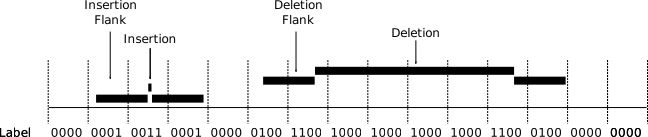
\includegraphics[width=1\textwidth]{figures/crf_labelling.pdf}
\caption{An example of the labeling scheme used for CRF model training and testing. Labels are a bitmask composed of variant and flanking information. First bit: Deletion. Second bit: Deletion Flank. Third bit: Insertion. Fourth bit: Insertion Flank.}
\label{crf_labels}
\end{figure}

We also had to choose what portions of the data to train the model on, since it would be unfeasible to train on the entire reference genome, and would likely bias the model against predicting any deletions because the vast majority of the reference does not participate in a deletion variant. First, we took all of the simulated insertion and deletion variants, and added regions of 250bp with the label ``Deletion Flank'' to either side. In addition, we selected 10,774 Cloudbreak calls. Some of these overlapped with the true variants, but the others added regions to the training set which had produced false positives. We then expanded all of the 9,497 regions selected for training by first adding 400bp to either end, and then adding the length of the resulting region to both sides. This ensured that all true variants and false positives were flanked by many windows that were properly labeled ``Outside Variant''.

To train our model, we coded it in Factorie and used their implementation of the LGBFS algorithm with L2 regularization. We also experimented with other optimizers including the online AdaGrad regularized dual averaging algorithm \cite{Duchi:2011:ASM:1953048.2021068} with L1 regularization but did not see large differences in preliminary testing. A limited difference in results on the test data combined with faster training times guided our choice of LGBFS; however, exploring different optimization methods with different feature sets could still be a useful area for research.

\section{Improving Cloudbreak Calls with CRF Predictions}

For our initial implementation, we adopted the approach of rapidly identifying candidate regions using a fast tool (Cloudbreak in this instance), adding flanking regions to them, and then running the CRF model on those candidate regions to try to label the true variants. Of course, this bounds the recall of the CRF approach to the recall of the candidate regions selected by the preliminary screen, but this strategy is far more than trying to label the entire genome.

For the test set, we used the same data set for individual NA18507 described in Section~\ref{section_na18507}, with 37X coverage by high-quality 100bp paired end reads with an insert size of 300bp. To choose regions to test on, we used Cloudbreak predictions for the same data set, at a low threshold to increase sensitivity. \todo{get actual number} We then created test windows to run inference on in the CRF model by again adding 200bp of flank to each side of each deletion prediction interval, and then adding the length of the interval in each direction. To conduct inference we use the Viterbi max-product belief propagation algorithm implemented in Factorie.

We then took all windows that the CRF model labeled deletions and merged contiguous blocks of windows to form intervals. For each such interval, we assign a confidence score as follows: first, for each window in the interval we calculate the sum of the likelihoods assigned to labels which indicate a deletion (i.e. have the ``Deletion'' bit set to one). We then compute the average of this window score across the entire deletion interval, giving us an overall CRF confidence in the deletion interval as a whole.

Finally, we refined the initial set of Cloudbreak deletion calls using the CRF calls according to the following rule: if a Cloudbreak deletion call and a CRF deletion call share a reciprocal overlap of at least 60\%, we consider that Cloudbreak call to be confirmed by the CRF model. By reciprocal overlap, we mean that 60\% of the length of the Cloudbreak call overlaps the CRF call, and 60\% of the CRF call overlaps the Cloudbreak call. For confirmed calls, we take the boundaries of the CRF deletion interval to be the deletion variant boundaries, and multiply the Cloudbreak deletion likelihood ratio by the CRF confidence score to get an adjusted confidence score for the confirmed call.

\section{Results}

Figure~\ref{roc_NA18507_with_crf} shows a ROC curve that compares the confirmed CRF calls with the other methods including Cloudbreak. The sensitivity of the merged CRF predictions is limited compared to the other methods. However, the updated score, which combines the Cloudbreak likelihood ratio with the CRF confidence, does provide a small improvement in discriminative power, as the true positives occur at higher thresholds than when using the unadjusted Cloudbreak score.

\begin{figure}
\centering
\includegraphics[width=\textwidth]{/Users/cwhelan/Documents/svpipeline/figures/NA18507_DELS_ROC_with_CRF.pdf}
\caption{ROC curve showing the accuracy of Cloudbreak calls that have been verified and refined with conditional random field predictions (Cloudbreak-CRF)}
\label{roc_NA18507_with_crf}
\end{figure}

Although the CRF method provides only a limited benefit to discriminative power over the raw Cloudbreak calls, it proves to be excellent at improving the breakpoint resolution of the calls. Figure~\ref{breakpoint_resolution_NA18507_with_crf} shows the breakpoint resolution of each of the methods, as reported previously in Chapter~\ref{chap_cloudbreak_eval}, with the addition the Cloudbreak calls confirmed by the CRF model. The confirmed calls have dramatically better resolution than the original Cloudbreak call set. With CRF confirmation, Cloudbreak's median difference between the true deletion length and the predicted length, 17bp, is now similar to that of DELLY-RP, which at 16bp is the best performing read-pair based method according to this metric (methods that take advantage of split-read mappings, such as DELLY-SR and Pindel, of course do better in this category). When one considers that Cloudbreak's predictions and the CRF features and labels are all based on the use of 25bp windows, it is clear that most of the time the CRF predictions are accurately identifying the window which contains the true breakpoint.

\begin{figure}
\centering
\includegraphics[width=.8\textwidth]{/Users/cwhelan/Documents/svpipeline/figures/breakpointResolutionNA18507_withCRF.pdf}
\caption{Breakpoint resolution of each tool's successful predictions on the NA18507 data set, including Cloudbreak calls which were verified and refined with CRF predictions (Cloudbreak-CRF)}
\label{breakpoint_resolution_NA18507_with_crf}
\end{figure}

\section{Features Selected by the CRF}

It can often be informative to examine the features that are given high scores by a machine learning technique. Table~\ref{crf_feature_selections} shows the top 25 features learned by the CRF for the window labels that correspond to ``Deletion Breakpoint'' (the windows which contain the endpoints of deleted regions) and ``Insertion''. Surprisingly, the CRF has learned a strong association between the deletion breakpoint label and the presence of simple repeats, showing how much correspondence there is between those features and the variants in the training set. As we might expect given the improvement in localizing breakpoint locations, soft clipping-related features are given high scores, particularly when it occurs in conjunction with coverage drops. The mu2 feature is used heavily for both deletions and insertions. Surprisingly, the Cloudbreak likelihood ratio does not occur often in the highest scoring features. Further examination of the feature scores may allow for improvements in feature engineering to create more parsimonious and effective models.

\begin{table}
\begin{centering}
\footnotesize
\resizebox{\textwidth}{!}{
\begin{tabular}{|lr|lr|}
\hline
\multicolumn{2}{|c|}{Deletion} &	\multicolumn{2}{c|}{Insertion} \\
Feature Name & Score & Feature Name & Score \\
\hline
simpleRepeat & 0.6 & softClip > 1.0 & 0.47 \\
260 < mu2 < 340 and simpleRepeat & 0.34 & simpleRepeat & 0.41 \\
simpleRepeat neighbor & 0.34 & softClip > 3.0 & 0.39 \\
rdepth < .1 and simpleRepeat & 0.32 & 260 < mu2 < 340 and softClip > 1.0 & 0.38 \\
260 < mu2 < 340 and simpleRepeat neighbor & 0.29 & softClip > 1.0 neighbor & 0.31 \\
softClip > 1.0 and covDrop20 > 5.0 & 0.23 & softClip > 2.0 & 0.29 \\
softClip > 3.0 and covDrop20 > 5.0 & 0.2 & mu2 < 260 in region & 0.26 \\
mu2 < 260 and lr = 0 in region & 0.19 & 260 < mu2 < 340 and softClip > 3.0 & 0.25 \\
softClip > 1.0 & 0.18 & rdepth < .1 and simpleRepeat & 0.24 \\
softClip > 3.0 and covDrop20 > 10.0 & 0.17 & rdepth > 1 and simpleRepeat neighbor & 0.23 \\
softClip > 2.0 and covDrop20 > 5.0 & 0.17 & softClip > 2.0 neighbor & 0.22 \\
mu2 > 340 and simpleRepeat & 0.17 & softClip > 1.0 in region & 0.22 \\
covDrop20 > 5.0 in region & 0.17 & mu2 < 260 and simpleRepeat & 0.21 \\
changePoint > 5.0 in region & 0.16 & simpleRepeat and repeat & 0.21 \\
softClip > 2.0 and covDrop20 > 10.0 & 0.15 & singletons > 1.0 and covDrop20 > 5.0 & 0.21 \\
covChangePoint > 10.0 in region & 0.15 & softClip > 2.0 in region & 0.2 \\
softClip > 1.0 neighbor & 0.14 & softClip > 3.0 neighbor & 0.2 \\
mu2 > 340 in region & 0.14 & 260 < mu2 < 340 and softClip > 2.0 & 0.2 \\
mu2 > 340 and lr > 0.75 & 0.14 & rdepth > 1 and simpleRepeat & 0.2 \\
changePoint > 15.0 and rdepth < .5 in region & 0.14 & softClip > 1.0 and rdepth > 1 & 0.16 \\
mu2 > 340 and softClip > 1.0 & 0.13 & mu2 < 260 neighbor & 0.16 \\
softClip > 1.0 and covDrop20 > 10.0 & 0.13 & lr > 0.75 and simpleRepeat & 0.15 \\
260 < mu2 < 340 and covDrop20 > 10.0 neighbor & 0.13 & 260 < mu2 < 340 and lr = 0 in region & 0.15 \\
rdepth < .1 and covDrop20 > 5.0 neighbor & 0.13 & softClip > 1.0 and repeat & 0.15 \\
rdepth < .25 & 0.13 & changePoint > 5.0 and softClip > 3.0 & 0.14 \\
\hline
\end{tabular}
}
\caption{Most important features learned by the CRF model for deletion and insertion breakpoints. ``Neighbor'': feature occurs in neighboring window. ``In region'': feature occurs within 300bp of current window. Feature names are the same as those in Table~\ref{crf_feature_definitions}}
\end{centering}
\label{crf_feature_selections}
\end{table}

\section{Discussion}

With the CRF model presented in this chapter, we have shown that the use of local features is a useful abstraction that can enable innovative algorithm approaches to the SV detection problem. We redefined SV detection as a sequence labeling problem, and created a framework for generating and managing local features across the genome that can integrate read pair, split read, and read depth related features, as well as features that incorporate prior knowledge such as genome annotations. Despite only training with simulated data that likely does not incorporate all of the aspects of the SV detection problem that make it difficult, we were able to generate useful predictions from our model.

Although the improvements in accuracy we achieved with the CRF model are marginal at best, it did prove to be very effective in improving Cloudbreak's breakpoint resolution, which was one of the weak points of the initial implementation of Cloudbreak as described in the previous chapters. The fact that for the majority of correctly predicted variants the CRF model was able to correctly identify the windows in which the breakpoint occurred indicates that the resolution could potentially be further improved with reductions in window size. In addition those windows identified could be excellent targets for exhaustive split read analysis or local assembly.

Opening the door to arbitrary features allows the potential to include a variety of types of information useful for SV detection in a single unified framework. There is the potential to use other types of genomic annotations that could be useful for detecting where the SV signals might be distorted due to sequence content. In this work we used binary features indicating the presence of repeats and segmental duplications. There are more fine-grained measures of repetitiveness and its effect on short read alignment, such as the genome mappability score \cite{Lee:2012bk} that could help to distinguish difficult regions. In addition, GC content in genomic sequence is known to have an effect on sequencing depth and copy number estimation \cite{Benjamini:2012er} and could be added as an additional feature to help correct for these biases. Another type of feature that similarly represents 'prior knowledge' and could be incorporated into this framework is sets of predictions from different SV detection tools. Finally, the SV detection methods that have achieved the greatest overall accuracy for non-cancer domains are those that pool multiple samples from across the same population, such as Genome STRiP~\cite{Handsaker:2011ki}. The pooled signals are used to identify candidate variant regions, which are then genotyped in each sample separately in a second pass over the data. These candidate variant regions could also be used as features within an integrated machine learning technique.

Finally, the characterization of the problem as a generic sequence labeling task over arbitrary features could potentially enable the use of a variety of different statistical and machine learning techniques for the SV detection problem in addition to the CRFs explored in this chapter. For example, deep learning techniques such as sequential deep belief networks~\cite{andrew2012:sdbn} have recently been used very successfully in sequence processing tasks in speech recognition and other domains. Since it is difficult to find fully annotated training data for the SV detection problem, the fact that deep learning networks are amenable to semi-supervised training with unlabeled data \cite{weston2012} makes them an attractive area for future research.

\chapter{Analysis of Evolutionary Breakpoint Features}
\label{chap_breakpoint_analysis}

This chapter genomic describes data analysis work unrelated to the algorithmic development of Cloudbreak and its extensions, although it is related at the biological level because it deals with genome breakpoints and rearrangements. It is important not only to be able to locate genomic breakpoints, but also to understand the genomic contexts in which they are located. As we discussed in Chapter~\ref{chap_background}, the sequence features of the genome that neighbor structural variations can leave clues about the mechanisms that caused the rearrangements, as in the cases of large homologies that point to the activity of non-allelic homologous recombination (NAHR) or the microhomologies that indicate non-homologous end joining (NEHJ). In this chapter we examine a set of structural variations that have reshaped a large genome at the evolutionary timescale: the chromosomal rearrangements of the gibbon genome. We analysed the locations in which the gibbon genome has been rearranged relative to humans and the other apes, first using a smaller set of breakpoint data, and then using the entire gibbon genome reference sequence created by the International Consortium for Sequencing and Annotation of the Gibbon Genome. The associations we discovered could help to provide insights into the mechanisms into which the gibbon genome was rearranged. \todo{and perhaps its structure and function}

\section{Background}

In Chapter~\ref{chap_background}, we mentioned that SVs can occur in the genomes of populations of cells at many different levels, ranging from the rearrangements that occur in populations of cells within a tumor in a single individual, to SVs that are polymorphic within the population of a species, and all the way to the structural differences between the genomes of different species. This last type of rearrangement represents SVs that occured within a population and then became fixed in that species and preserved as the species evolved and differentiated. 

Rather than identifying them by comparing short-read sequencing data to a reference genome, as has been the focus of the previous chapters, we can detect these evolutionary breakpoints by directly comparing the genomes of species to each other. In the past this was done by mapping the location of individual genes to particular chromosomes; with the advent of whole genome sequences they be found by conducting sequence alignments (or multiple sequence alignments) of the the reference genomes for the species under study. When species share regions that contain the same genes and other genomic features, in the same order, it is referred to as \emph{shared synteny}. By examining the endpoints of syntenic blocks of the genomes of two species, or \emph{synteny breakpoints}, it is possible to find the breakpoints of the structural variations that rearranged the structure of the two genomes.

Identifying evolutionary breakpoints can give insights into the mechanisms of their formation. It was long thought that chromosomal breakpoints were largely random, such that they are equally likely to occur at any location in the genome~\cite{Ono:1973tr,Nadeau:1984tm}. Higher-resolution analysis, however, revealed that certain regions of the genome are much more likely to give rise to evolutionary breakpoints~\cite{Pevzner:2003ba}, and this result was re-confirmed once whole-genome reference sequences for many species became available~\cite{Murphy:2005hv}. Tantalizingly, Murphy et al. also showed that these reused evolutionary breakpoint regions overlapped significantly with the breakpoints of SVs found in cancer genomes~\cite{Murphy:2005hv}.

This raises the question of whether these regions of the genome have special properties that make them more likely to be observed participating in evolutionary breakpoints. In Chapter~\ref{chap_background}, we described the fact that certain mechanisms for SV formation, in particular NAHR, are a result of having regions with high sequence similarity at different locations in the genome, as the cell's machinery attempts to repair double-stranded breaks in DNA by joining homologous regions together. As one might expect if evolutionary breakpoints were the result of NAHR, a large number of chromosomal rearrangements in mammals, approaching 40\%, are associated with segmental duplications\cite{Bailey:2004fb,Bailey:2006fn}. Closer examination of breakpoints from a variety of species, including human, chimp, macaque, rat, mouse, pig, cattle, dog, opossum, and chicken, confirmed that they contain more sequence that is not unique relative to the rest of the genome than would be expected by chance, including segmental duplications (SDs) and other low-copy number repeats~\cite{Larkin:2009ij}. However, analysis of evolutionary sequence divergence in these repeats indicates that some of the duplications may have occured after the rearrangements, casting dobt on the theory that an NAHR-like process is primarily responsible~\cite{Bailey:2004fb}, and indeed the precise mechanisms behind evolutionary breakpoints remain unknown.

Gibbons represent a unique opportunity to study the process of evolutionary genomic rearrangement because of their highly rearranged genomes. In most branches of the evolutionary tree, large genomic rearrangements are rare events, occurring at a rate of approximately two every ten million years~\cite{Wienberg:2004gt}. However, some species have appear to have faster or slower rates of rearrangments. For example, the orang-utan genome has very few medium and large scale rearrangements relative to the expected number given its time of evolutionary divergence~\cite{Locke:2011gn}. At the other end of the spectrum, gibbon genomes have 10 to 20 times more rearrangements than would be expected given the rate in other mammals, and in fact the four genera of gibbons have numbers of chromosomes ranging from 28 to 52, suggesting that gibbon genome has been shuffled rapidly since it diverged from the other apes 17 to 18 million years ago~\cite{Misceo:2008kg}.

Given their highly rearranged karyotypes, gibbons represent an excellent model in which to study mechanisms of chromosomal rearrangements. Until recently, however, the whole genome sequence of the gibbon was not available. Therefore, several studies analyzed gibbon genome breakpoints using techniques involving bacterial artificial chromosomes (BACs)~~\cite{Girirajan:2009kw,Carbone:2006jk,Carbone:2009p1012}. BACs are medium sized (150-350kb) fragments of DNA from a sample that are isolated, turned into plasmid bacterial chromosomes, and then amplified in a culture. By probing gibbon BACs with arrays or testing their hybridization to human chromosomes using flourescent \emph{in situ} hybridization experiments, it is possible to isolate BACs which span human-gibbon evolutionary breakpoints. This allows one to locate the breakpoint regions to within several hundred kb, and the small size of the BACs relative to the entire genome makes them much easier to sequence, allowing the analysis of sequence features near the breakpoints. Initial studies examined selected BACs from the northern white-cheeked gibbon species \emph{Nomascus leucogenys leucogenys} (NLE) and found a high level of segmental duplications and repetitive sequence at the breakpoints~\cite{Carbone:2006jk,Roberto:2007dt}. Similar results were found in BACs from the white-handed gibbon species \emph{Hylobates lar} (HLE)~\cite{Misceo:2008kg}. A later study increased the scope by examining 24 sequenced NLE BACs that spanned breakpoints, and analyzed gibbon-specific insertions of repeats and segmental duplications at the breakpoints to postulate several possible rearrangement mechanisms~\cite{Girirajan:2009kw}. More recently, Carbone et al.~\cite{Carbone:2009p1012} analyzed 57 NLE BACs and, in addition to segemental duplications, found enrichment for \emph{Alu} repetititve elements. The latter study also found differences in CpG methylation marks on \emph{Alu} elements near the breakpoints, suggesting that there may be an epigenetic process involved in gibbon genomic rearrangements.

\section{Evolutionary Breakpoints in the Gibbon Genome determined by BACs}

To determine whether or not the characteristics observed in the breakpoints identified by BACs from NLE and HLE gibbons were generalizable to the entire gibbon family, we conducted an expanded analysis of gibbon breakpoints based on the sequencing of additional BACs covering breakpoints in the gibbon genera \emph{Symphalangus} and \emph{Hoolock} using samples from the species \emph{Symphalangus syndactylus} (SSY) and \emph{Hoolock leuconedys}. Since each of the gibbon genera has a different karyotype, identifying breakpoints across all four allows for greater insight into the mechanisms and timing of the evolution of the gibbon family. I contributed to this research by anlayzing the overlap between breakpoints from all four gibbon genera with genomic features. This work was published by Capozzi et al.~\cite{Capozzi:2012bb}.

\subsubsection{Methods}

To search for genomic features potentially associated with gibbon chromosomal breakpoints we computed the significance of the overlap between gibbon evolutionary breakpoint regions and a set of genomic features of interest using permutation tests. The purpose of the permutation analysis is to discover the null distribution for the number of overlaps a set of intervals has with a particular feature in the genome. In essence, the test asks: if my intervals were placed in random locations on the genome, what is the probability of seeing the number of overlaps we observed with that features in the actual data? 

To conduct the test, while maintaining the chromosomal assignment and length of break- point regions, we permuted their start coordinates 10,000 times using BEDTools version 2.16.2~\cite{Quinlan:2010km}. Genomic regions annotated as centromeres and telomeres in the ``Gaps'' track of the hg19 build were excluded from possible random placements of the regions. Locations of the features were held constant. We then compared the number of features that overlapped a breakpoint region to the observed distribution of results among the randomly permuted regions, and used the quantile of the real observed value in that distribution as an estimate of the P-value of observing a value equal to or greater than the real observation. In order to be able to conduct a large number of permutations to determine a true background distribution for each feature, we created a pipeline for distributing the permutations across a compute cluster using the grid management system HTCondor.

The analysis was performed on the human hg19 assembly. The features examined were genes, human segmental duplications, and some repeat families (Alu, LINE, ERV, and SVA). We also investigated the associations between breakpoint regions and chromatin structure by testing the overlap with open chromatin regions in human embryonic stem cells reported by the ENCODE consortium~\cite{ENCODEProjectConsortium:2011iz}. 

\subsubsection{Results}

We found a significant enrichment for genes (Bonferroni adjusted P-value = 0.0287), human segmental duplications (P = 0.0366), Alu (P < 0.0001), and SVA (P = 0.0008) (Figure~\ref{gibbon_bac_permutations}). We did not find significant enrichment for LINE and ERV repeats, nor for the ENCODE open chromatin regions. Systematically shifting the location of breakpoint regions by increments of 10 kb up- and downstream of their actual location, up to a maximum of 1 MB, shows that the locations of the breakpoint regions gives the greatest or close to the greatest number of overlaps with the four significantly overlapping features (genes, segmental duplications, Alu, and SVA) in the local genomic neighborhood, also shown in Figure~\ref{gibbon_bac_permutations}.

\begin{figure}
\centering
\includegraphics{figures/gibbon_bac_permutations.jpg}
\caption{Enrichment of genomic features in breakpoint regions. Permutation tests were used to assess the overlap between the gibbon breakpoints and genomic features. (A) Segmental duplications; (B) Alu elements; and (C) SVA elements. The black vertical line indicates the observed value for the breakpoints identified in the study. In all three cases it is evident that the genomic features have a higher overlap with the breakpoints than one could expect by chance.}
\label{gibbon_bac_permutations}

\end{figure}

\section{Analysis of Breakpoints from the Gibbon Genome Reference Sequence}

Continuing the work I have already done in analyzing the evolutionary breakpoints mapped with the gibbon BAC clones, I am working with the International Consortium for Sequencing and Annotation of the gibbon genome to analyze the additional breakpoints discovered through the assembly of the gibbon reference genome. To do so, I am conducting additional association tests with a variety of features. One of these features is a set of binding sites of the evolutionarily conserved binding factor CTCF, which I have identified through the analysis of chromatin immunoprecipitation followed by sequencing (ChIP-seq) data. CTCF has recently been shown to be associated with the three-dimensional structure of DNA and chromatin in the cell~\cite{Dixon:2012gc}, and therefore may have important associations with genomic DNA breakpoints and structural variations.

\todo{I am also helping to analyze the breakpoints from a set of over forty mesenchymal tumor samples in which genomic rearrangements have created ring-shaped chromosomes. The breakpoints that cause these chromosomal rearrangements cluster into several frequently broken areas. I am currently working on analyzing these breakpoint regions using my permutation analysis pipeline in order to determine genomic features that may be significantly associated with these breakpoints, including repeat elements, open chromatin sites and other data from ENCODE, and binding motifs for enzymes known to be involved with breakpoint formation.}

\section{Breakpoints in the gibbon genome reference}

\subsection{Overlap with genomic features: repeats and genes}

To analyze the enrichment of genomic features in the regions flanking evolutionary breakpoints, we used a permutation based approach. The number of overlaps between breakpoint flanks and each feature of interest in the assembled genome (the observed overlap count) was compared to a background distribution calculated by randomly permuting the locations of breakpoint regions 100,000 times. The Nleu1.1 version of the assembly was used for these analyses. For our breakpoint regions, we chose those breakpoints for which we had single nucleotide resolution, and added flanking regions to either side of the breakpoint; in breakpoints in which the breakpoint fell within a gibbon-specific repeat element, we chose the flanking regions of the repeat. In each permutation, the location of each breakpoint region was randomly changed, while keeping the length and scaffold assignment of the breakpoint region the same. We then counted the number of overlaps between the randomized breakpoint regions and the feature of interest (the permuted overlap count). Enrichment p-values were computed as the proportion of permuted overlap counts that were more extreme than the observed overlap count. We also visualized the spatial relationship of breakpoint regions to each type of figure by simultaneously shifting the locations of the breakpoint regions up to 1MB in each direction, in increments of 25kb, and counting the proportion of shifted breakpoint regions that overlapped a feature of interest, after discarding regions that were shifted beyond the beginning or end of a scaffold. Permutation testing and shift testing were carried out using custom Python scripts and the BEDtools~\cite{Quinlan:2010km}, pybedtools\cite{Dale:2011cl}, and BEDOPS~\cite{Neph:2012kq} libraries; the code is publicly available at \url{https://github.com/cwhelan/permuting-feature-enrichment-test}.

We tested for enrichment in the breakpoint regions of the following features: genes, segmental duplications, and several classes of repetitive elements: Alu, L1, LAVA, and LTR. In addition to testing the entire Alu family, we also tested the subfamilies AluS, AluJ, and AluY individually. Gene locations were taken from Ensembl build 70. For the segmental duplication analysis, we used the segmental duplications identified by the WSSD method (Section S3). Alu, L1, and LTR locations were identified using RepeatMasker output. In order to determine the distance from the breakpoints at which enrichments are strongest, we varied the size of the breakpoint flanking regions by adding differently sized intervals; we tested flanking regions of size 100bp, 250bp, 500bp, and 1000bp. We corrected for multiple testing using the FDR under dependency method of Bejamini and Yekutieli~\cite{Benjamini:2001fs}. Breakpoint regions are depleted for genes, but enriched for Alu elements and segmental duplications (Extended data figure 2). The enrichment for Alu is primarily due to a strong enrichment of the AluS subfamily.Even though genes were depleted overall, some of the genes overlapping with breakpoints belong to interesting biological categories (Table ST5.1 ).

In addition to testing the count of overlaps between breakpoint flanking regions and repeats, we also conducted a complementary test that examined the distance of each breakpoint to the nearest repeat of a given class. For this test we used only the 44 breakpoints for which we had single nucleotide breakpoint resolution, with no Gibbon-specific repeats directly intersecting the breakpoint. We compared these breakpoint locations to 10,000 randomly selected regions in the Nleu1.0 genome, selected using the randomBed program from the BEDTools suite. The distance to the nearest repeat for either the breakpoints or random positions was determined using BEDTools closestBed.  We compared the distribution of distances to a repeat for the breakpoints to the distribution of distances to a repeat for the 10,000 randomly selected positions using the Kolmogorov-Smirnov (K-S) test. We examined the distance to any repeat, as well as those for Alu, LINE, and LTR elements, and finally the AluJ, AluS, and AluY subfamilies. After FDR correction for multiple hypothesis testing, the distance test showed similar results to the overlap test described above, with signficant results for the Alu family as a whole, and for the AluJ and AluS subfamilies, indicating that the breakpoints tend to be closer to those repeats than random locations in the genome.

Breakpoint regions were simultaneously shifted in increments of 25kb, up to a maximum of 1MB in each direction, and the proportion of breakpoint regions that overlap a feature of interest is reported. Shifts show that breakpoints are centered on regions that are depleted in genes but close to regions that contain genes, while the opposite is true for segmental duplications. Alu elements are more evenly spread across the shift regions (Extended data figure 2).

\subsection{Overlap with CTCF binding sites}

\subsubsection{Chromatin Immunoprecipitation (ChIP) sequencing for CTCF}

CTCF ChIP-seq assays were performed according to Schmidt et al.~\cite{Schmidt:2012dt} on eight EBV-transformed lymphoblastoid cell lines established for the same individuals used for the diversity panel (Table ST2.1). In brief, CTCF-bound DNA was immunoprecipitated using an Anti-CTCF rabbit polyclonal antibody (07-729, Millipore). End-repair was performed on immunoprecipitated and input DNA prior to A-tailing and ligation to single-end Illumina sequencing adapters. DNA was amplified using Illumina primers 1.1 and 2.1 in an 18-cycle PCR reaction. Gel electrophoresis was used to select 200-300 bp DNA fragments. DNA libraries were sequenced using 36 bp reads on an Illumina Genome Analyser II according to the manufacturer’s instructions.

\subsubsection{Peak calling from CTCF ChIP-seq Data}

We aligned reads to the nomLeu2 reference using BWA (version 0.62)~\cite{Li:2009p836} with default parameters, and removed non-uniquely mapping reads. We then called peaks using CCAT~\cite{Xu:2010fu}, with parameters fragmentSize 100, slidingWindowSize 150, movingStep 10, isStrandSensitiveMode 1, minCount 10, minScore 4.0, and bootstrapPass 50. We then combined the peaks called across the different individuals and chose the following set for further analysis: any peak called in an individual individual by CCAT with an FDR of less than 0.05, as well as any peak that was called in more than one individual with an FDR of less than 0.1. (Table ST5.2)

\subsubsection{Determination of Gibbon-specific and shared CTCF binding sites}

Gibbon peaks were classified as shared or gibbon-specific by comparing them to a set of CTCF peaks called on human, macaque, and orangutan individuals (Schwalie, P.C. et al. under review). First, orthologous locations of gibbon CTCF peaks in other primate species were determined using a local installation of the Ensembl Compara multi-species alignment database (http://uswest.ensembl.org/info/docs/api/compara/index.html). This database contains alignments of the references for human (GRCh37), chimp (CHIMP2.1.4), gorilla (gorGor3.1), orangutan (PPYG2), rhesus macaque (MMUL\_1), and gibbon (Nleu1.1). A multi-species alignment of each Gibbon CTCF peak region was generated in paml format. Gibbon CTCF peaks for which no multi-alignment were present, or where the nucleotide alignment identity to human and macaque was less than 70\%, were excluded from analysis. We then created a non-redundant list of non-gibbon CTCF peaks by converting the human, orangutan and macaque peaks to gibbon coordinates using the Compara database, and then merging the results using the mergeBed tool from the BEDTools suite to remove redundant entries. Shared and gibbon-specific CTCF peaks were then identified as those gibbon CTCF peaks that did or did not intersect a peak in the non-redundant list of non-gibbon CTCF peaks.

\subsubsection{Analysis of CTCF peaks in relationship with gibbon-human synteny breakpoints}

We identified 52,685 CTCF binding sites. Because of CTCF's function as an insulator and its known association with the boundaries of DNA topological domains~\cite{Dixon:2012gc}, we tested the overlap of CTCF binding sites and the gibbon synteny breakpoint regions. We find that 12 of the 1kb regions flanking breakpoints overlap with CTCF binding sites (one example showed in Extended data figure 2). Using the same permutation analysis described above, this overlap has an enrichment p-value of 0.0009. This effect was even stronger when we expanded the breakpoint flanking regions to 25kb,  as 95 expanded flanking regions overlap CTCF peaks for an enrichment p-value <0.0001 (Extended data figure 2).

We then tested whether the CTCF peaks causing the enrichment in breakpoint regions are specific to gibbons. Using CTCF ChIP-seq data for samples from human, macaque, and orangutan individuals, we classified CTCF binding sites as unique to gibbons (11,449 sites) or shared with a primate ancestor (41,236 sites). We found that the gibbon breakpoint regions are heavily enriched for CTCF binding sites shared with a primate ancestor (enrichment p-value = 0.0006) but are not significantly enriched for gibbon-specific CTCF binding sites. Again, the enrichment is stronger in the 25kb expanded breakpoint regions (enrichment p-value <0.0001) for shared binding sites, but not for gibbon-specific binding sites. This suggests that the formation or selection of gibbon genome rearrangements was associated with ancestral CTCF binding sites.

\chapter{Future Work}
\label{chap_future_work}

There are many possible extensions that could be made to enhance Cloudbreak's effectiveness as a general SV analysis tool for high-throughput sequencing data. However, implementing all of them is outside of the scope of this thesis, which aims to demonstrate the general effectiveness of a distributed computing approach to SV detection. These other extensions include:

\begin{itemize}
 \item Detection of additional SV types such as longer deletions, inversions, and translocations. While these would be useful and necessary additions to a complete variant detection pipeline, I believe that by showing the applicability of MapReduce to two classes of variants (short-to-midsize deletions, and short insertions), Cloudbreak will create a base from which to implement many additional SV detection algorithms in the future.
 \item Addition of a local assembly step to increase breakpoint resolution and validate SV candidates. Cloudbreak's breakpoint resolution is less than that of many other RP and SR algorithms. One approach to improving breakpoint resolution, and providing additional validation of predicted results, is to attempt to conduct a \emph{de novo} assembly of the reads that mapped near the breakpoints and their pairs. If effectively implemented, this would be a very useful addition to any SV detection algorithm. However, the implementation of such an approach in a distributed setting would likely be embarrassingly parallel, with multiple instantiations of a self-contained assembly algorithm run on different compute nodes. Therefore, it would not necessarily add to the demonstration of the effectiveness of the MapReduce framework to this domain.
 \item Incorporation of split-read signals into the Cloudbreak implementation. As sequencing technology improves, read lengths will continue to lengthen, making split-read mapping a more effective strategy for SV detection. Therefore, we have considered adding a split-read mapping algorithm to Cloudbreak as well. However, as with local assembly discussed above, non-distributed split-read aligners run in parallel for different subsets of the input reads would likely be just as effective. In addition, I believe that my formulation of SV detection based on genomic features could be extended to include a new set of features created by executing split-read mappers, especially in the context of the machine-learning approaches described above.
\end{itemize}

In summary, rather than providing a broad but shallow implementation of many possible application features, I believe that the demonstration of a system that leverages cluster and cloud computing to achieve state-of-the-art accuracy and runtime performance on a subset of the SV detection problem will provide a higher impact to the genomic sequencing research community.



% The library likes numbers rather than the `alpha' style.
\bibliographystyle{acm}
% Single space the bibliography to save space.
\begin{singlespace}
%\bibliography{thesis}
\end{singlespace}
%\printbibliography

% The appendices are optional, but they must follow the references.
%\appendix

% This section (the final one) contains a biographical note.
%
%\vita
%This section contains a biographical note.
%The following information (in essay form) should be contained in this section:
%place of birth; date of birth; schools attended; degrees awarded; areas of
%special interest; relevant profession experience; awards and honors; list
%of publications.

\end{document}
